% small.tex
\documentclass{beamer}
%\usetheme{default}
\usetheme{Warsaw}
\usecolortheme{whale}
\usepackage{tikz}
\usepackage[absolute,overlay]{textpos}
\usepackage{soul}
\usepackage{pdfpages}
\usepackage[most]{tcolorbox}
%\usepackage{multirow}
\usepackage{tikz,amsmath,array}
\usepackage{hyperref}

\newcommand{\greekbf}[1]{\boldsymbol{\mathrm{#1}}}
\newcommand{\btVFill}{\vskip0pt plus 1filll}
\newcolumntype{P}[1]{>{\centering\arraybackslash}p{#1}}

%\setbeamertemplate{background}[grid][step=.25\textwidth]

\title[fvhsgrhhfdss]{Reconstructing prehistoric human demography using end-to-end Bayesian analysis of radiocarbon dates}
%\subtitle
\author{Michael Holton Price}
\institute[SFI] {
	Santa Fe Institute\\
	MichaelHoltonPrice@gmail.com\\
	\line(1,0){0}\\
	Radiocarbon Universe Webinar Series\\
	09 Jun 2020\\
}
%\date{05 Feb 2014}
\date{}

% Note: default dimensions are 128 mm by 96 mm (4 x 3)
\begin{document}

%----------- titlepage ----------------------------------------------%
\begin{frame}[plain]
  \titlepage
\end{frame}

%----------- slide --------------------------------------------------%
\begin{frame}
  \frametitle{Accessing presentation and code}
  \centering
  https://www.overleaf.com/read/TEXT-AT-BOTTOM
  
\includegraphics[height=.85\textheight]{qr-code.png}
\end{frame}

%----------- slide --------------------------------------------------%
\begin{frame}[c]
    \frametitle{Follow Along / Run the Code Yourself}
    \centering
    \Large
      \href{https://www.overleaf.com/read/fvhsgrhhfdss}{https://www.overleaf.com/read/fvhsgrhhfdss}
      
    % This presentation is version controlled at:
    % https://github.com/MichaelHoltonPrice/radiocarbon_universe_2020_06_09
      
      \bigskip
      
      \href{https://github.com/eehh-stanford/baydem}{https://github.com/eehh-stanford/baydem}
      
      \bigskip
        
      \href{https://github.com/eehh-stanford/price2020}{https://github.com/eehh-stanford/price2020}
\end{frame}

%----------- slide --------------------------------------------------%
\begin{frame}
  \frametitle{Problem Statement}
    \begin{center}
      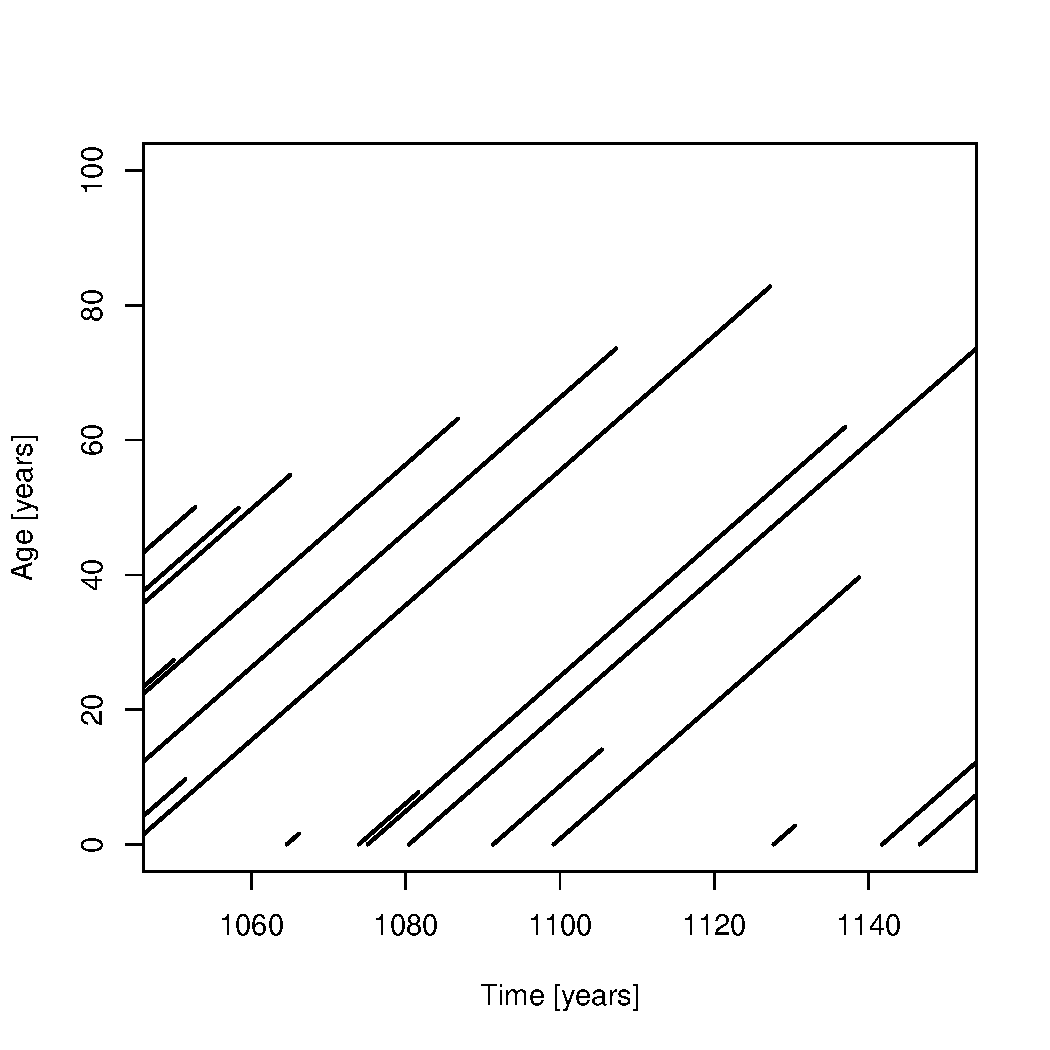
\includegraphics[height=.85\textheight]{lifeline_plot_no_horiz_line.pdf}
    \end{center}
\end{frame}

%----------- slide --------------------------------------------------%
\begin{frame}
  \frametitle{Problem Statement}
    \begin{center}
      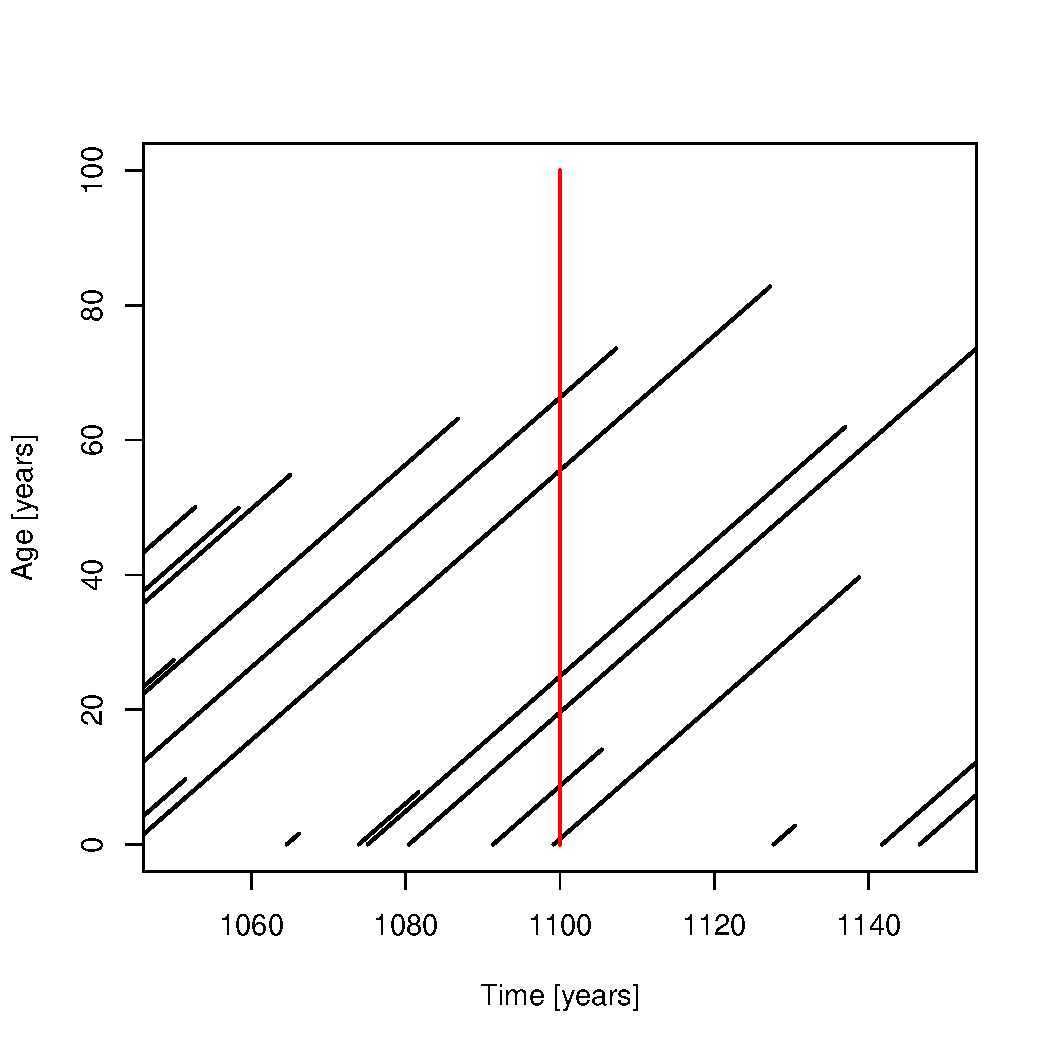
\includegraphics[height=.85\textheight]{lifeline_plot.pdf}
    \end{center}
\end{frame}

%----------- slide --------------------------------------------------%
\begin{frame}
  \frametitle{Geographic Scale}
  \begin{columns}[c]
   \column{.5\textwidth}
     \begin{block}{Site Demography}
      \begin{center}
        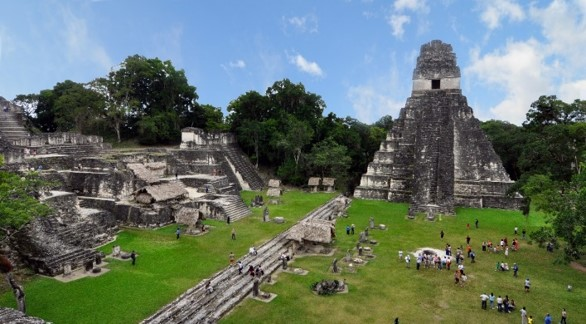
\includegraphics[width=1\textwidth]{maya_site.jpg}\
      \end{center}
    \end{block}
    \pause

   \column{.5\textwidth}
     \begin{block}{Regional Demography}
      \begin{center}
        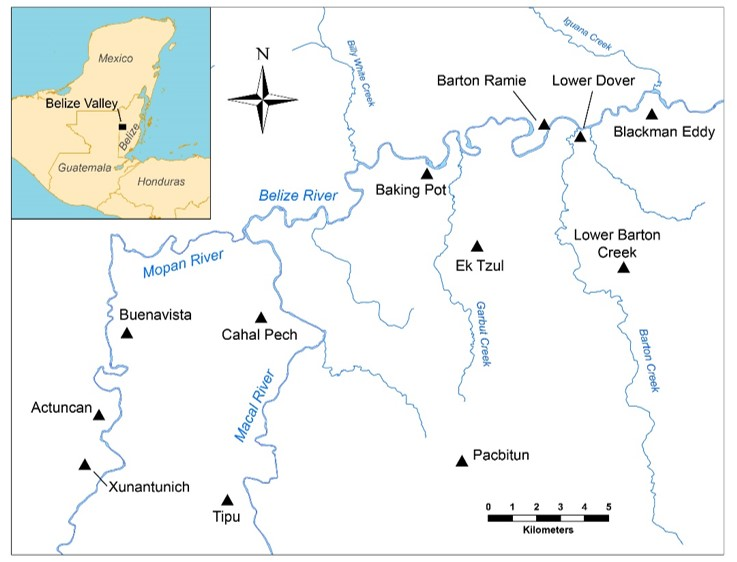
\includegraphics[width=1\textwidth]{belize_region.jpg}\
      \end{center}
    \end{block}
  \end{columns}

  \btVFill
  \small Images courtesy Julie Hoggarth \normalsize
\end{frame}

%----------- slide --------------------------------------------------%
\begin{frame}[t]
  \frametitle{Relevant Data}
  \begin{columns}[c]
   \column{.5\textwidth}
     \begin{block}{Direct}
     \begin{itemize}
       \pause
       \item{Date of Death [C14]} 
       \pause
       \item{Age at Death} 
       \pause
       \item{Isotopes} 
       \pause
       \item{DNA} 
     \end{itemize}
     \end{block}
    \pause

    \column{.5\textwidth}
     \begin{block}{Indirect}
     \begin{itemize}
       \pause
       \item{Pottery} 
       \pause
       \item{Charcoal} 
       \pause
       \item{House Counts} 
       \pause
       \item{etc.} 
     \end{itemize}
     \end{block}
  \end{columns}
\end{frame}

%----------- slide --------------------------------------------------%
\begin{frame}[t]
  \frametitle{A Tale of Two Problems: The Bias Problem}
  \pause
  \begin{itemize}
    \item A living population generates dateable material.
    \pause
    \item The amount of material is proportional to population size.
    \pause
    \item The material gets deposited in recoverable contexts.
    \pause
    \item Geological and taphonomic processes filter the material that persists to the present.
    \pause
    \item Archaeological sites are identified via survey, construction, or other means.
    \pause
    \item Archaeologists choose to excavate some of those sites.
    \pause
    \item A subset of dateable material is in fact dated.
    \pause
    \item A subset of dates are published or otherwise available for meta-analysis. 
    \pause
  \end{itemize}
\end{frame}

%----------- slide --------------------------------------------------%
\begin{frame}[t]
  \frametitle{A Tale of Two Problems: The Summary Problem}
  \pause
  \begin{itemize}
    \item Summed probability densities (SPDs) are the dominant, current method of summarizing sets of radiocarbon dates
    \pause
    \item SPDs are fundamentally flawed
    \pause
    \item A principled solution of the summary problem must be end-to-end
  \end{itemize}
\end{frame}

%----------- slide --------------------------------------------------%
\begin{frame}[t]
  \frametitle{Bayesian Inference on a Single Sample}
    \begin{center}
      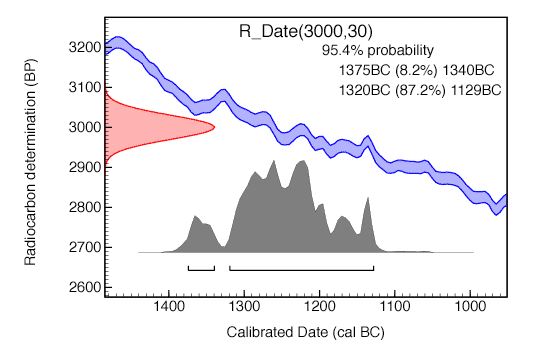
\includegraphics[height=.8\textheight]{calibration.png}
	\begin{textblock*}{100pt}(0pt,240pt)
      		\small OxCal Website \normalsize
	\end{textblock*}
    \end{center}
\end{frame}

%----------- slide --------------------------------------------------%
\begin{frame}[t]
  \frametitle{Bayesian Inference on a Single Sample: Uniform Prior}
    \begin{center}
      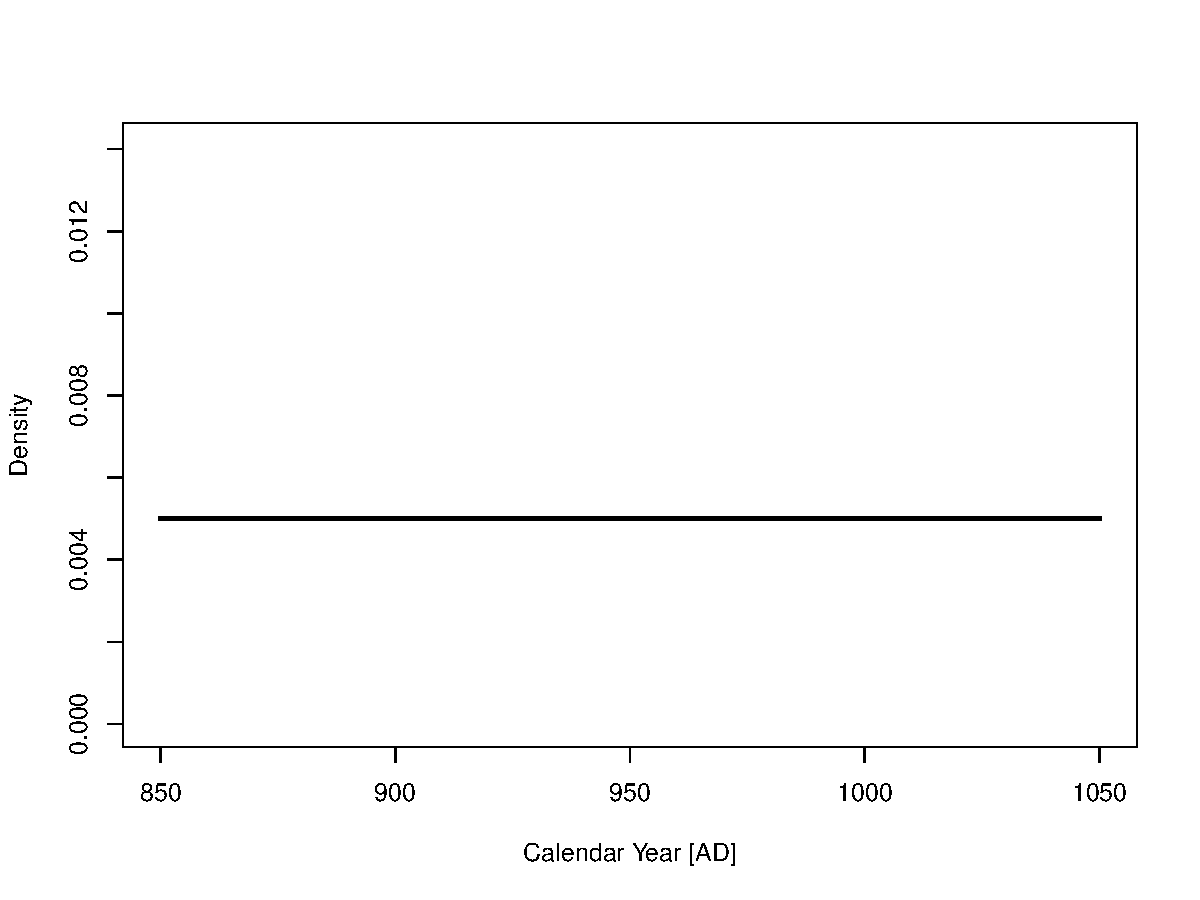
\includegraphics[height=.8\textheight]{single_obs_inf_plot1.pdf}
    \end{center}
\end{frame}

%----------- slide --------------------------------------------------%
\begin{frame}[t]
  \frametitle{Bayesian Inference on a Single Sample: Uniform Prior}
    \begin{center}
      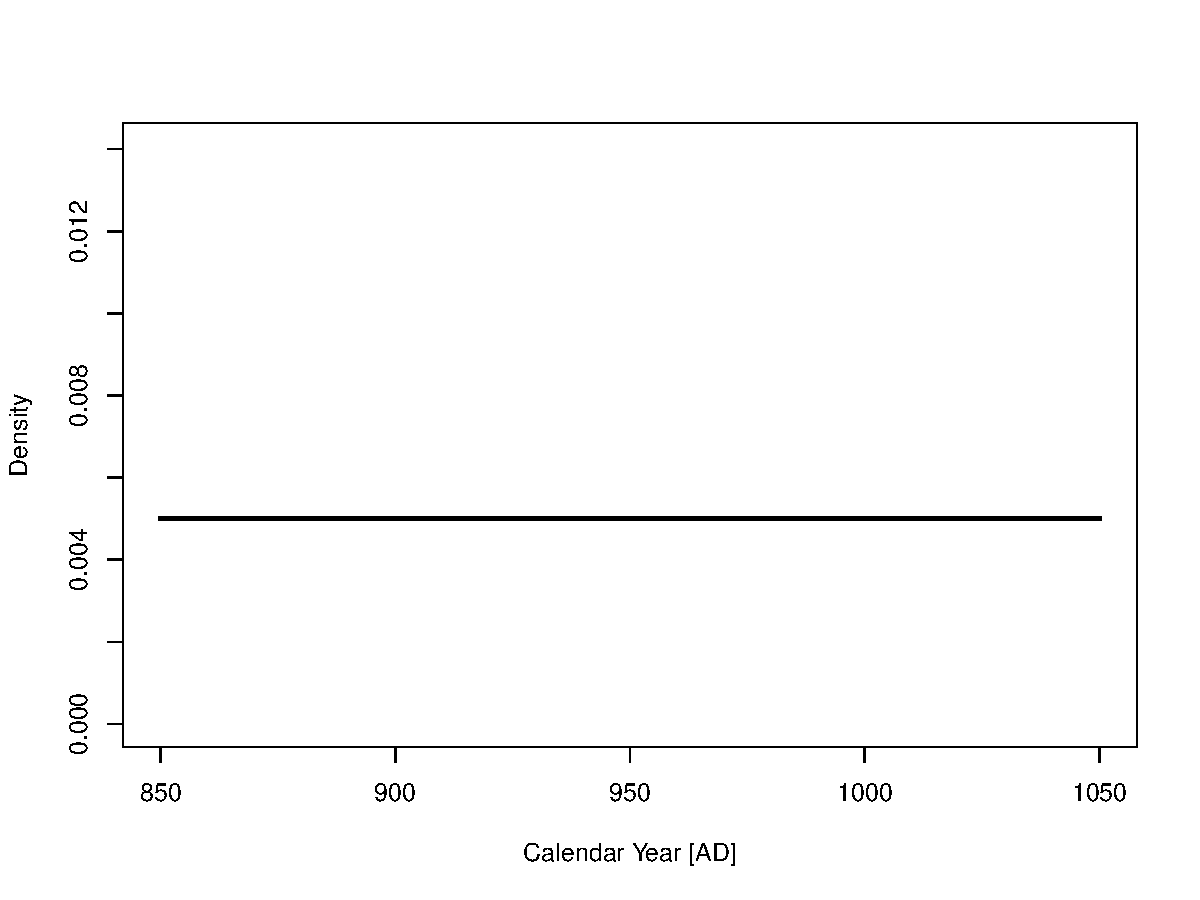
\includegraphics[height=.8\textheight]{single_obs_inf_plot1.pdf}
    \end{center}
    \begin{textblock*}{100pt}(175pt,140pt)
      \Large $p(t)$ \normalsize
	\end{textblock*}
\end{frame}

%----------- slide --------------------------------------------------%
\begin{frame}[t]
  \frametitle{Bayesian Inference on a Single Sample: Update}
    \begin{itemize}
    \item Radiocarbon determination
    \pause
    \item Calibration curve
    \pause
    \item Other constraints (for multiple samples, stratigraphy)
    \end{itemize}
\end{frame}

%----------- slide --------------------------------------------------%
\begin{frame}[t]
  \frametitle{Representing the radiocarbon determination}
    \begin{itemize}
    \item Uncalibrated years BP
    \item $t_{m}$
    \pause
    \item Uncertainty, uncalibrated years BP
    \item $\sigma_{t_m}$
    \pause
    \item Fraction Modern
    \item $\phi_m = \exp(-\frac{t_m}{\kappa})$
    \item $\sigma_m = \sigma_{t_m} \frac{\phi_m}{\kappa}$
    \item $\kappa=8033$
    \end{itemize}
 
\end{frame}

%----------- slide --------------------------------------------------%
\begin{frame}[t]
  \frametitle{Calibration Curve}
    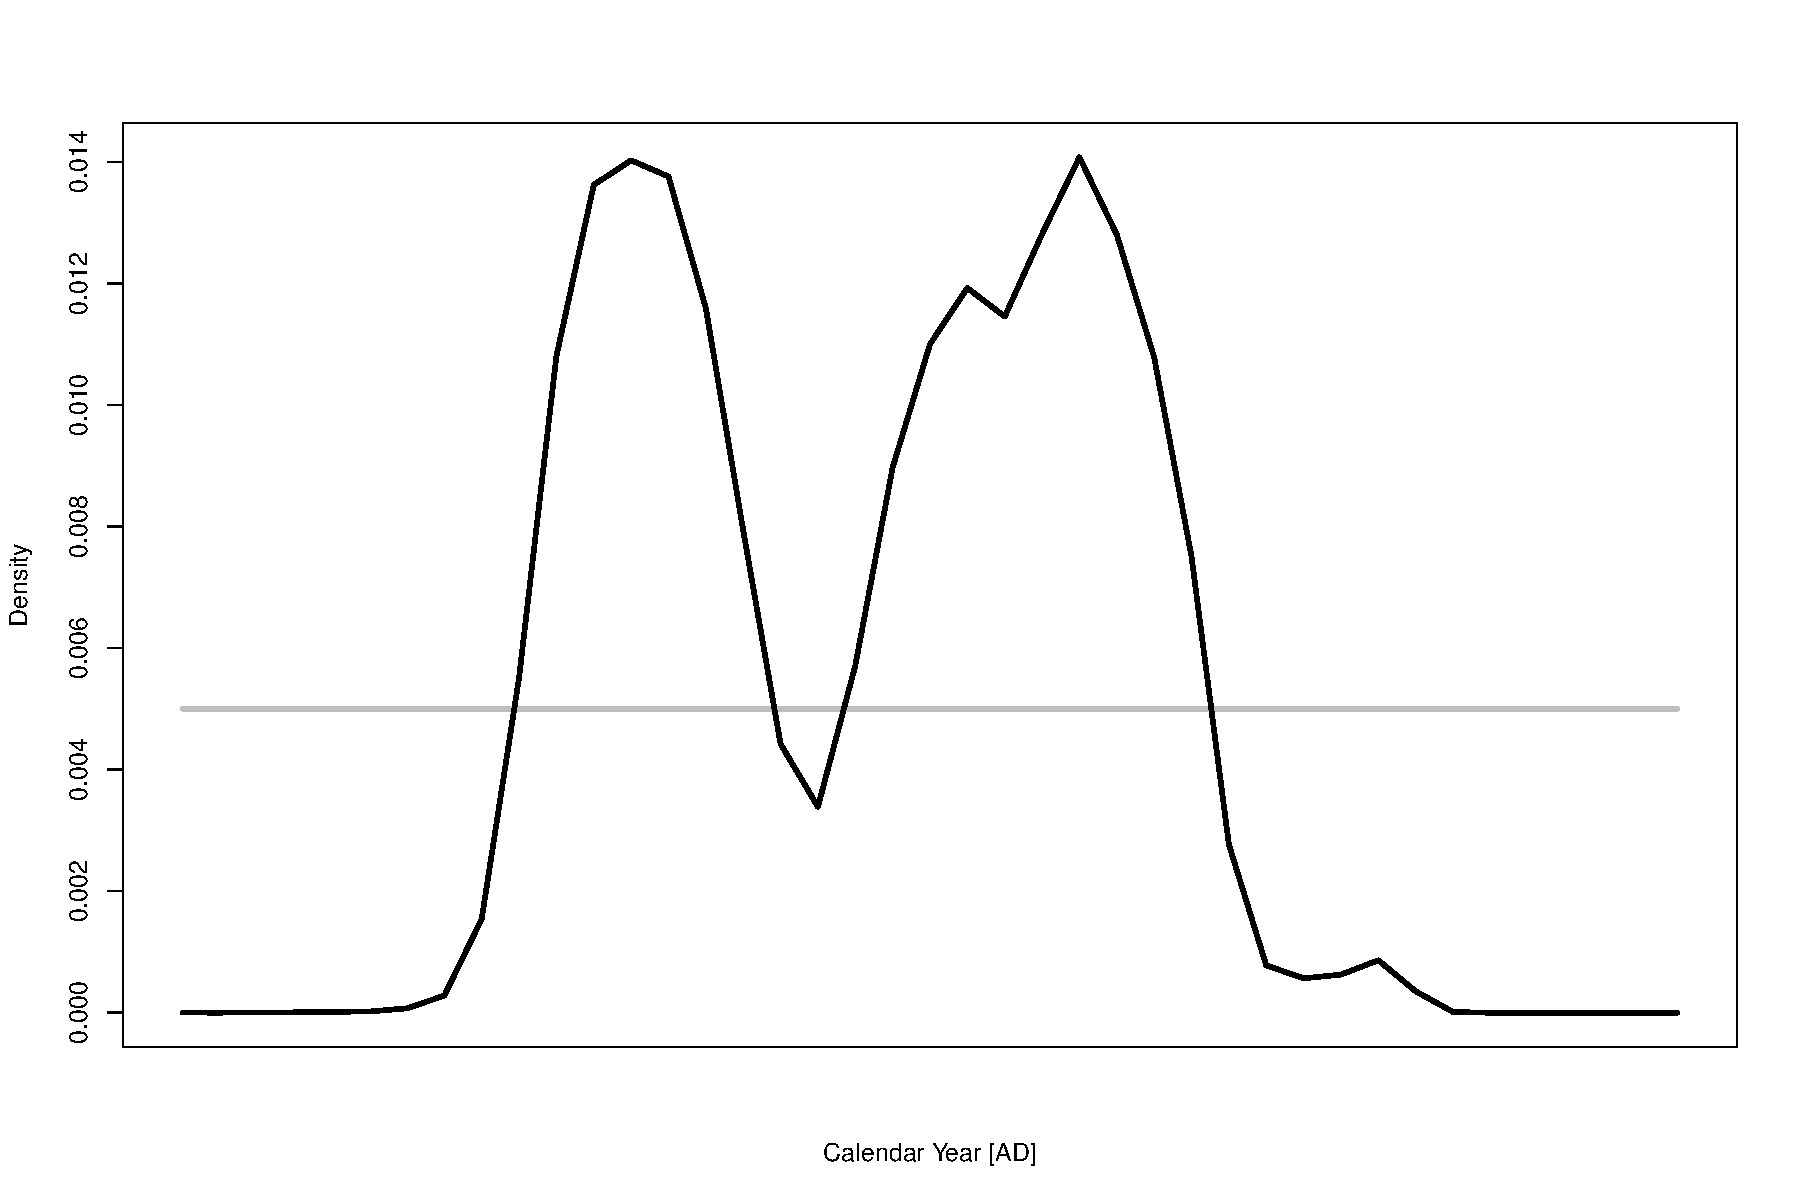
\includegraphics[height=.85\textheight]{single_obs_inf_plot2.pdf}
\end{frame}

%----------- slide --------------------------------------------------%
\begin{frame}[t]
  \frametitle{Calibration Curve}
    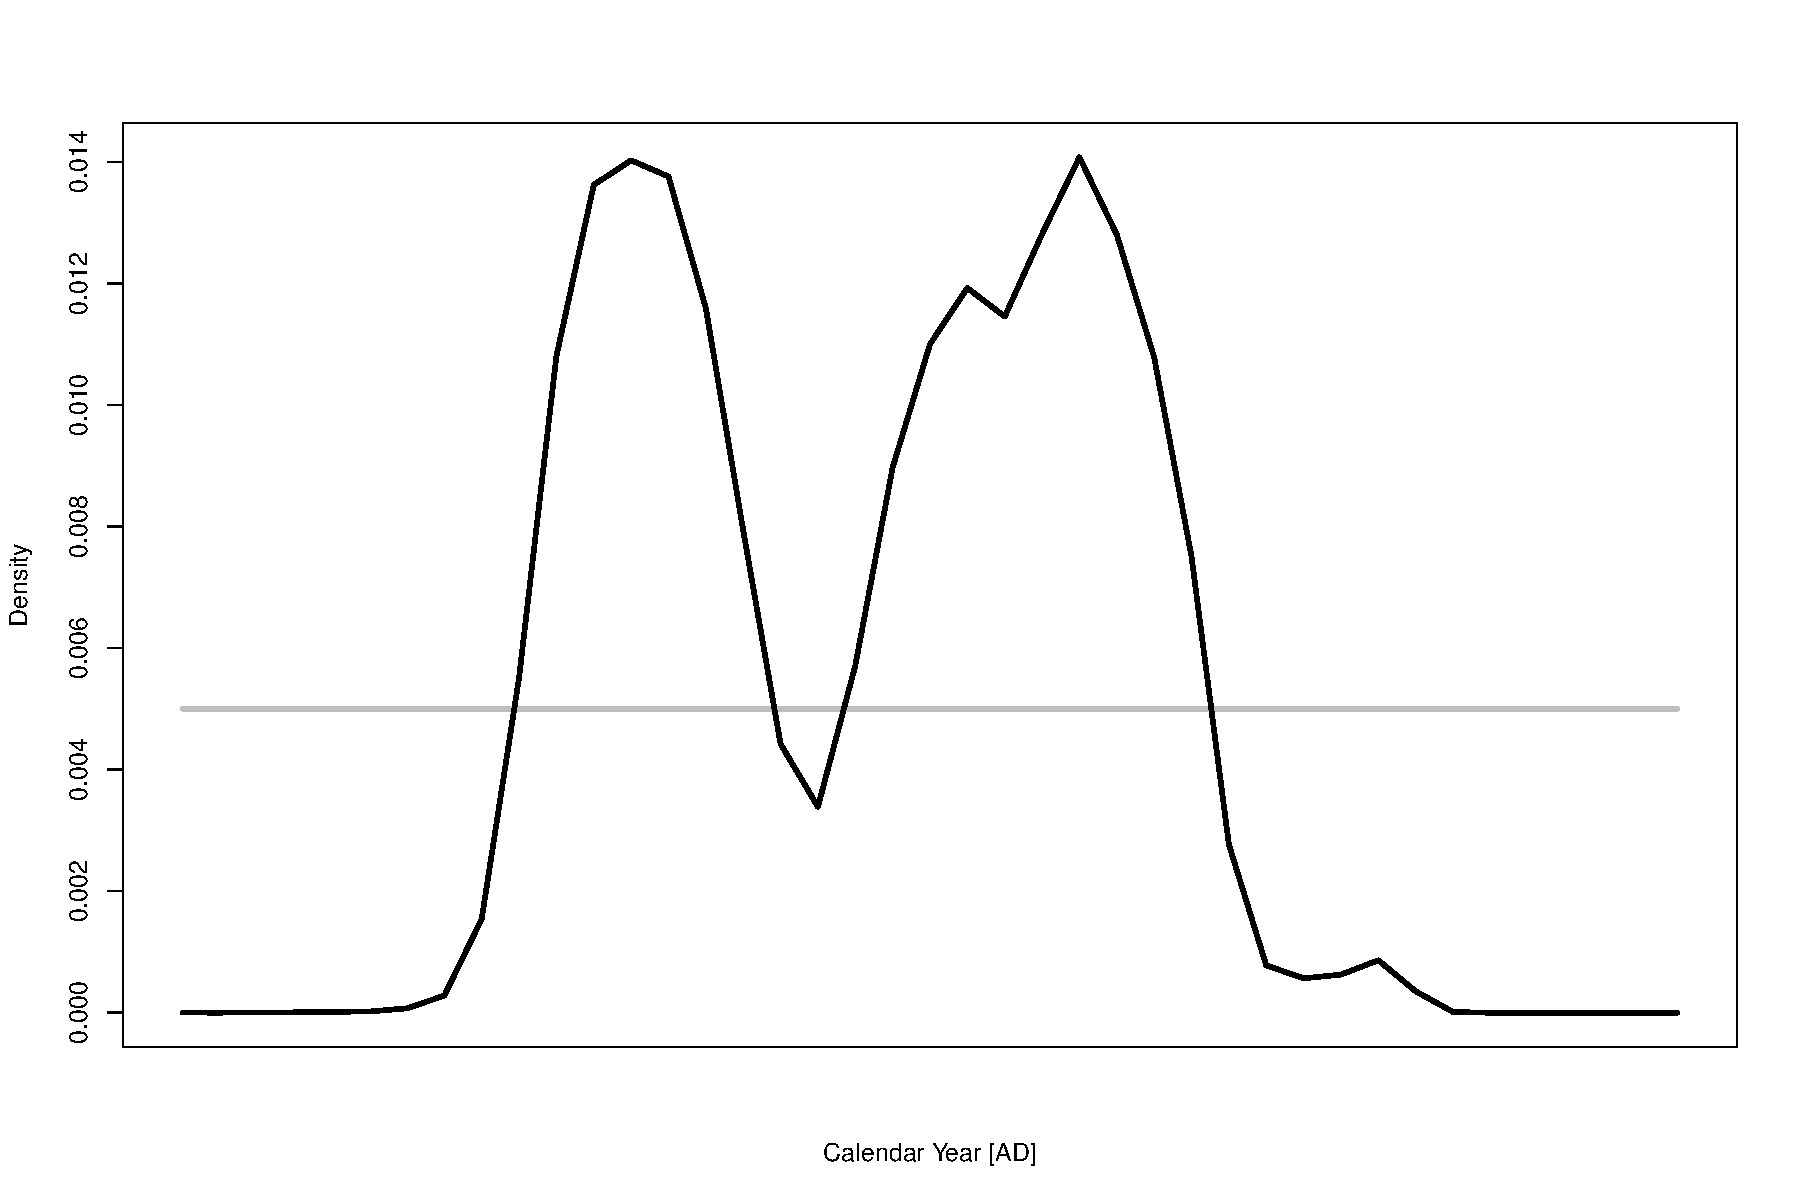
\includegraphics[height=.85\textheight]{single_obs_inf_plot2.pdf}
    \begin{textblock*}{100pt}(125pt,135pt)
      \Large $\phi_c(t)$ \normalsize
	\end{textblock*}   
\end{frame}

%----------- slide --------------------------------------------------%
\begin{frame}[t]
  \frametitle{Calibration Curve}
    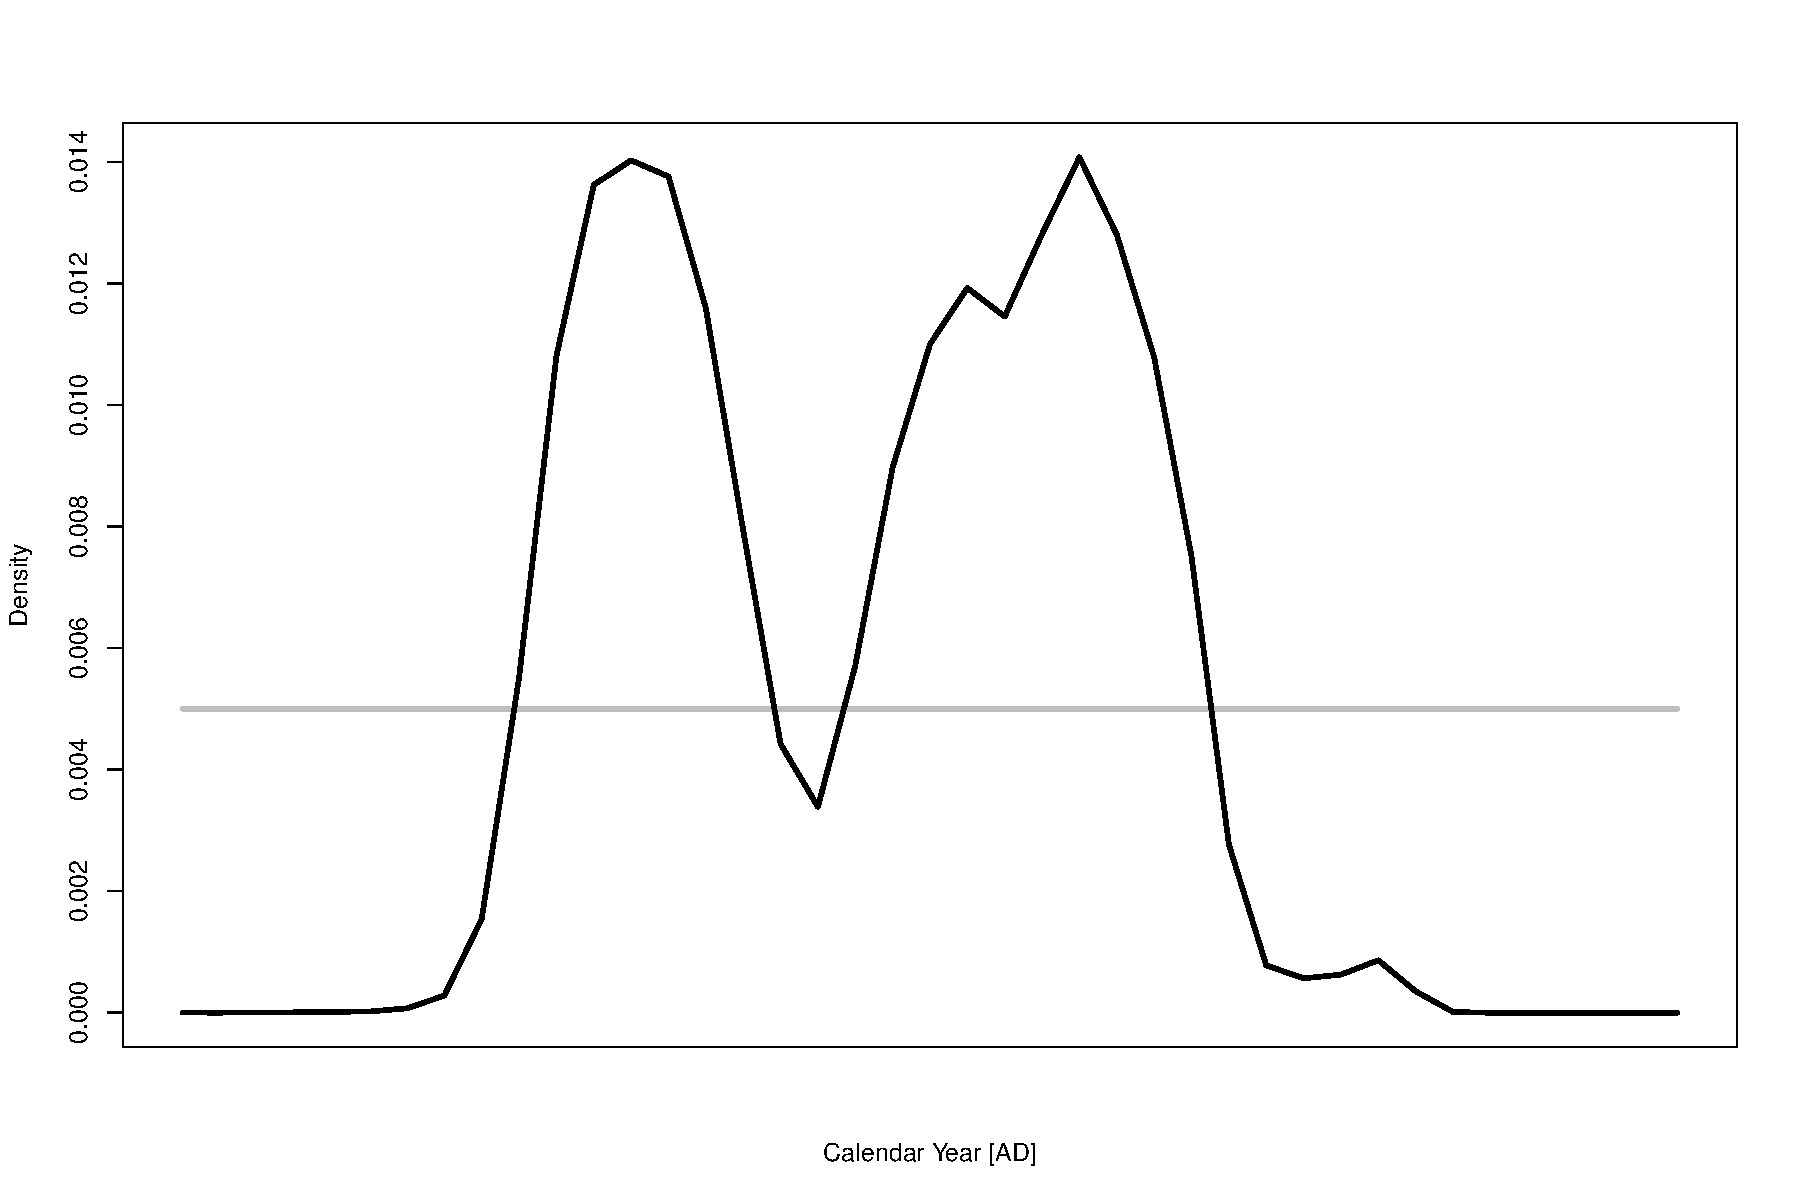
\includegraphics[height=.85\textheight]{single_obs_inf_plot2.pdf}
    \begin{textblock*}{100pt}(125pt,135pt)
      \Large $\phi_c(t)$ \normalsize
	\end{textblock*}   
    \begin{textblock*}{100pt}(125pt,185pt)
      \Large $\sigma_c(t)$ \normalsize
	\end{textblock*}   
\end{frame}

%----------- slide --------------------------------------------------%
\begin{frame}[t]
  \frametitle{Likelihood (single observation, given $t$)}
  \Large
  \begin{equation}
    \phi_m|t \sim N(\phi_c(t),\sigma^2(t))
  \end{equation}
  
  \bigskip
  
  \begin{equation}
    \sigma^2(t) = \sigma^2_m + \sigma^2_c(t)
  \end{equation}
  
  \bigskip
  
  \begin{equation}
    p(\phi_m|t) = \frac{1}{\sqrt{2\pi}\sigma(t)}\exp{(-\frac{1}{2}\frac{[\phi_m-\phi_c(t)]^2}{\sigma^2(t)})}
  \end{equation}
 
  \normalsize
\end{frame}

%----------- slide --------------------------------------------------%
\begin{frame}[t]
  \frametitle{Update (single observation, given $t$)}
  \Large
  \begin{equation}
    p(t|\phi_m) \propto p(\phi_m|t) p(t)
  \end{equation}
  \normalsize
\end{frame}

%----------- slide --------------------------------------------------%
\begin{frame}[t]
  \frametitle{Update (single observation, given $t$)}
    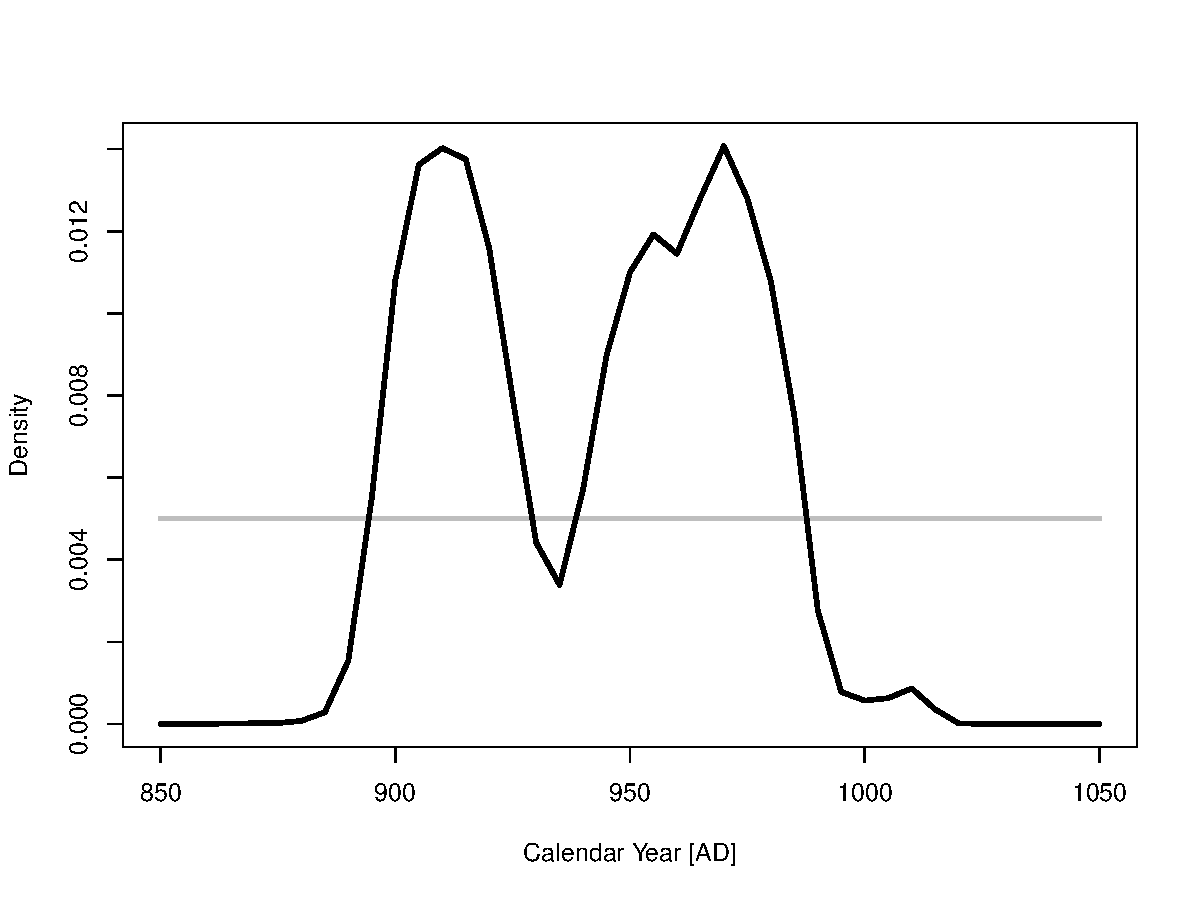
\includegraphics[height=.85\textheight]{single_obs_inf_plot3.pdf}
    \begin{textblock*}{100pt}(175pt,140pt)
      \Large $p(t)$ \normalsize
	\end{textblock*}
    \begin{textblock*}{100pt}(220pt,80pt)
      \Large $p(t|\phi_m)$ \normalsize
	\end{textblock*}
\end{frame}

%----------- slide --------------------------------------------------%
\begin{frame}[t]
  \frametitle{Summed probability densities (SPDs)}
    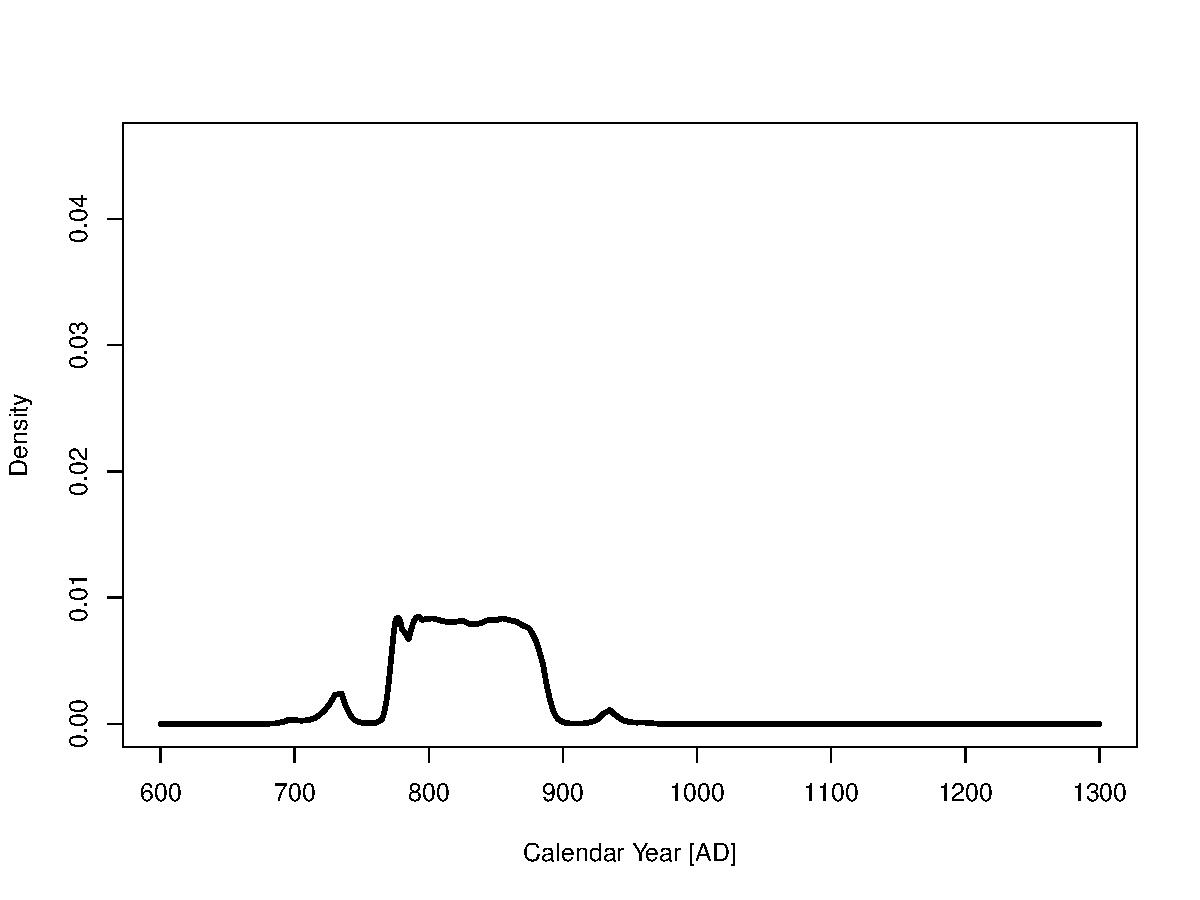
\includegraphics[height=.85\textheight]{spd1.pdf}
\end{frame}

%----------- slide --------------------------------------------------%
\begin{frame}[t]
  \frametitle{Summed probability densities (SPDs)}
    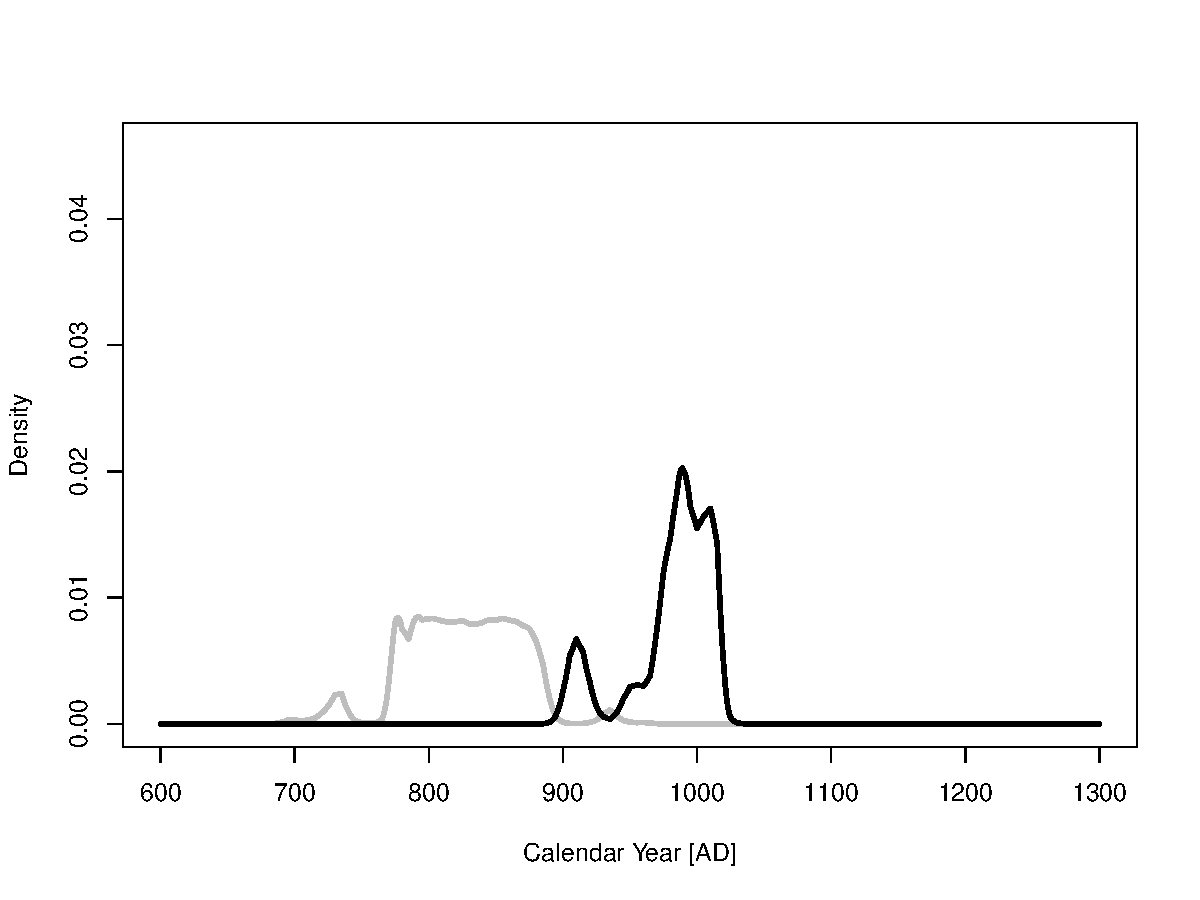
\includegraphics[height=.85\textheight]{spd2.pdf}
\end{frame}

%----------- slide --------------------------------------------------%
\begin{frame}[t]
  \frametitle{Summed probability densities (SPDs)}
    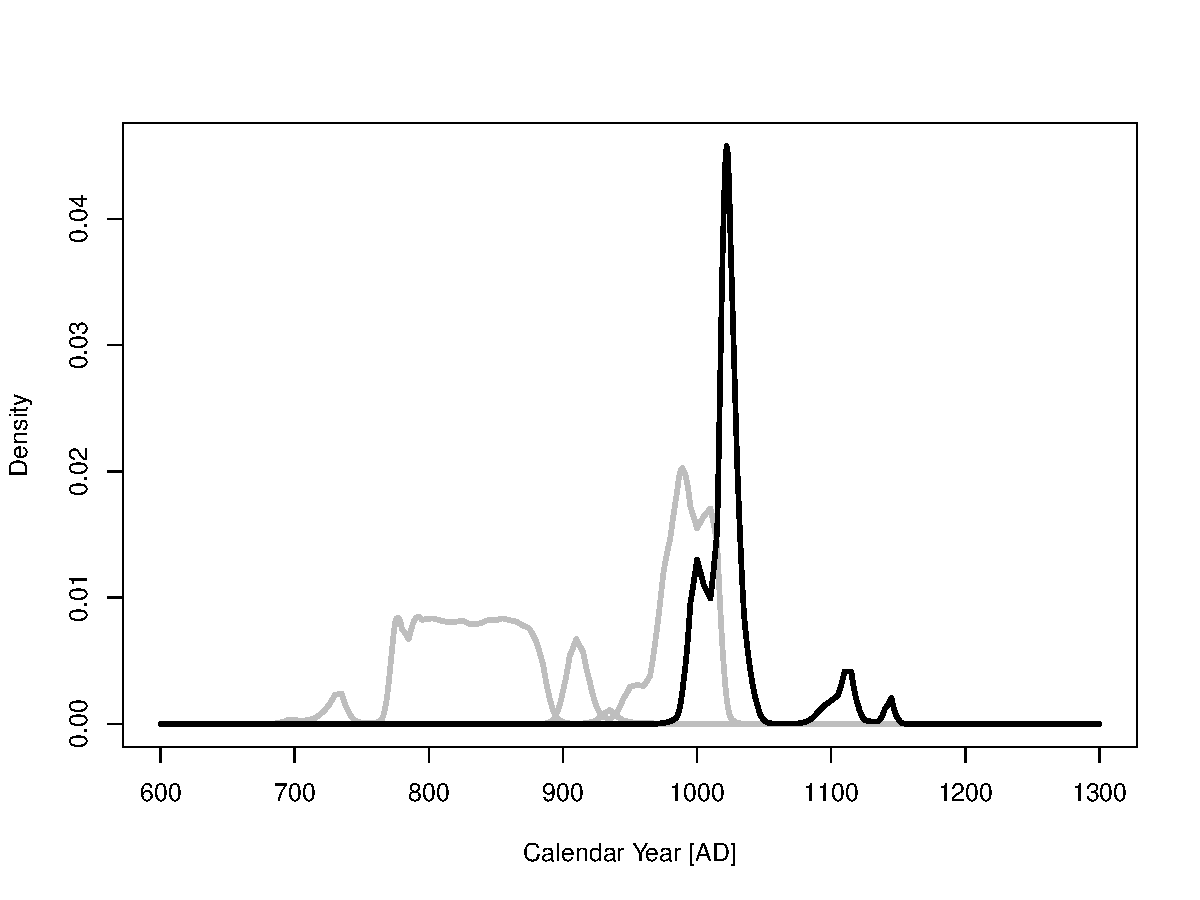
\includegraphics[height=.85\textheight]{spd3.pdf}
\end{frame}

%----------- slide --------------------------------------------------%
\begin{frame}[t]
  \frametitle{Summed probability densities (SPDs)}
    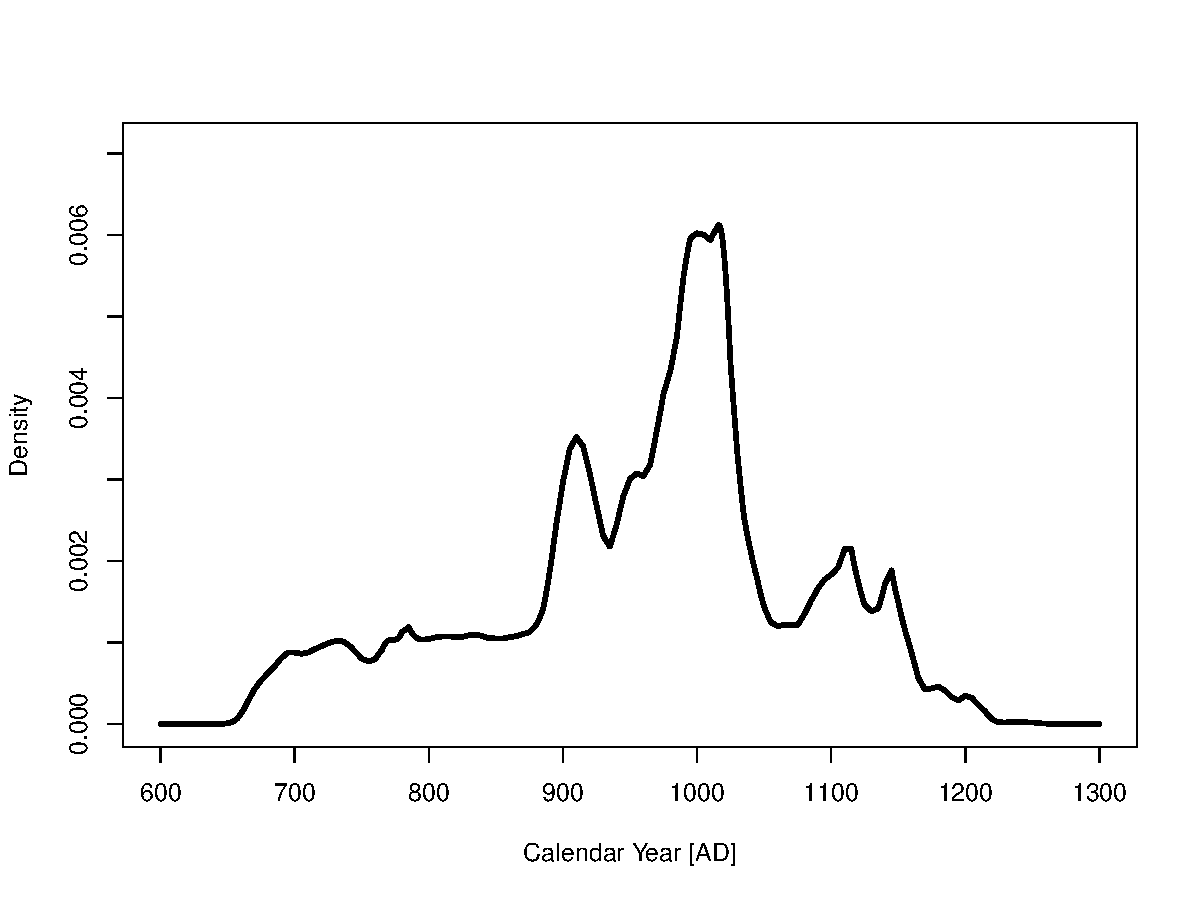
\includegraphics[height=.85\textheight]{spdall.pdf}
\end{frame}

%----------- slide --------------------------------------------------%
\begin{frame}[t]
  \frametitle{Summed probability densities (SPDs)}
    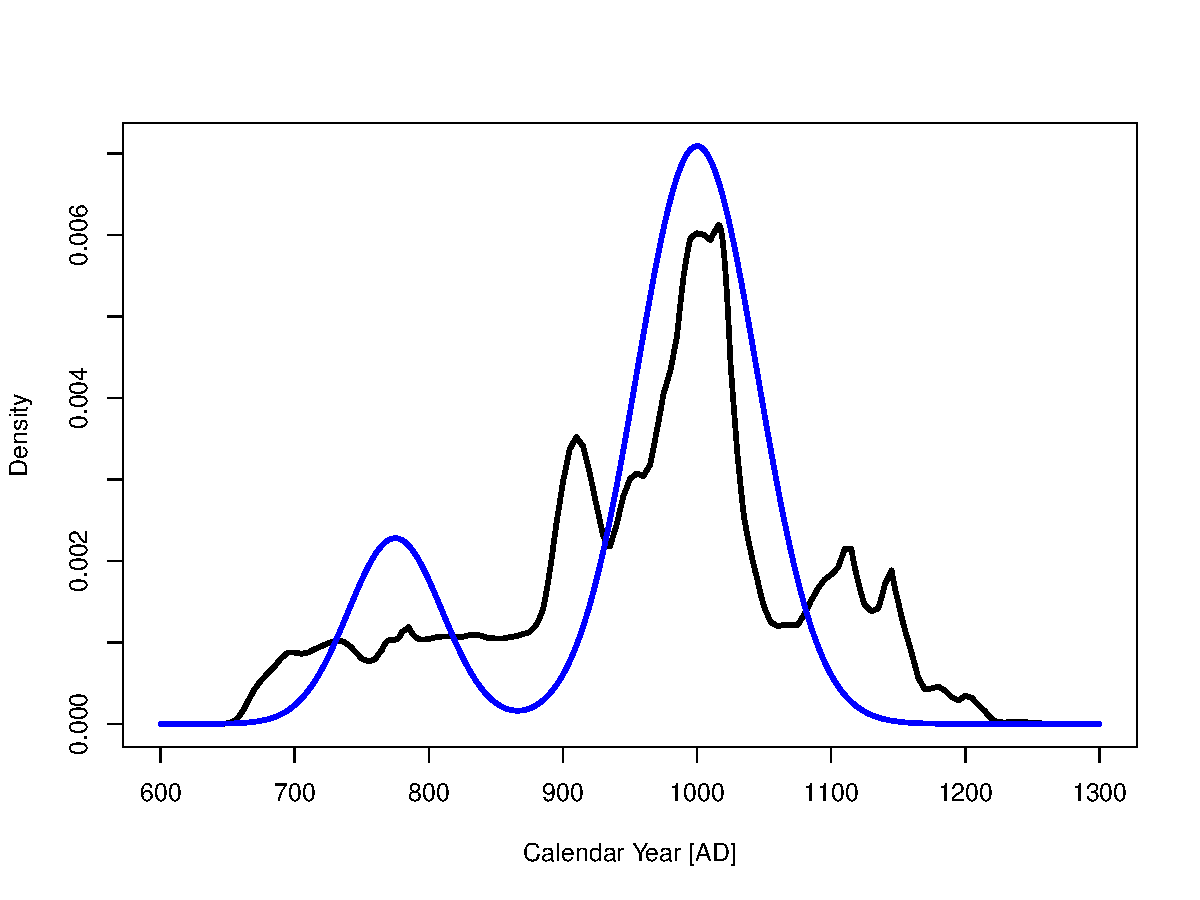
\includegraphics[height=.85\textheight]{spdall_sim.pdf}
\end{frame}

%----------- slide --------------------------------------------------%
\begin{frame}[t]
  \frametitle{Fundamental flow of inference: SPDs}
    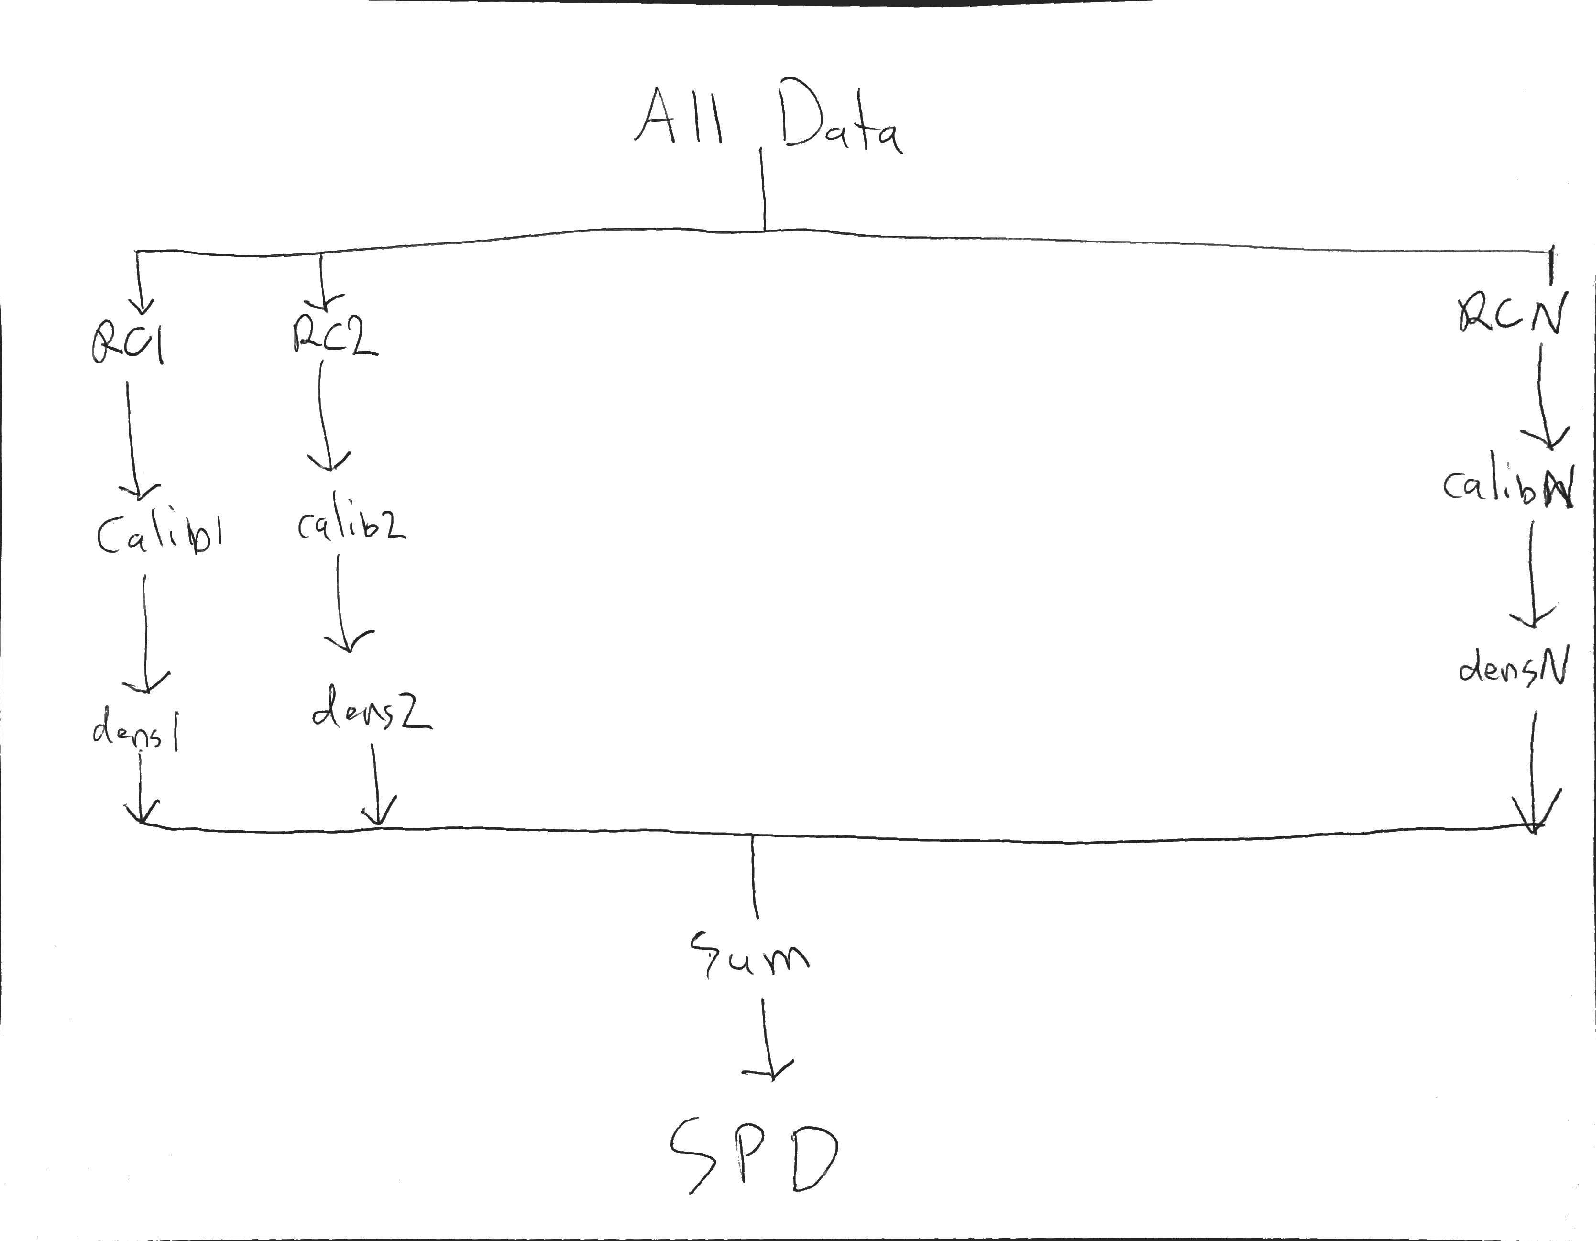
\includegraphics[height=.85\textheight]{spd_flow.pdf}
\end{frame}

%----------- slide --------------------------------------------------%
\begin{frame}[t]
  \frametitle{Fundamental flow of inference: End-to-End}
    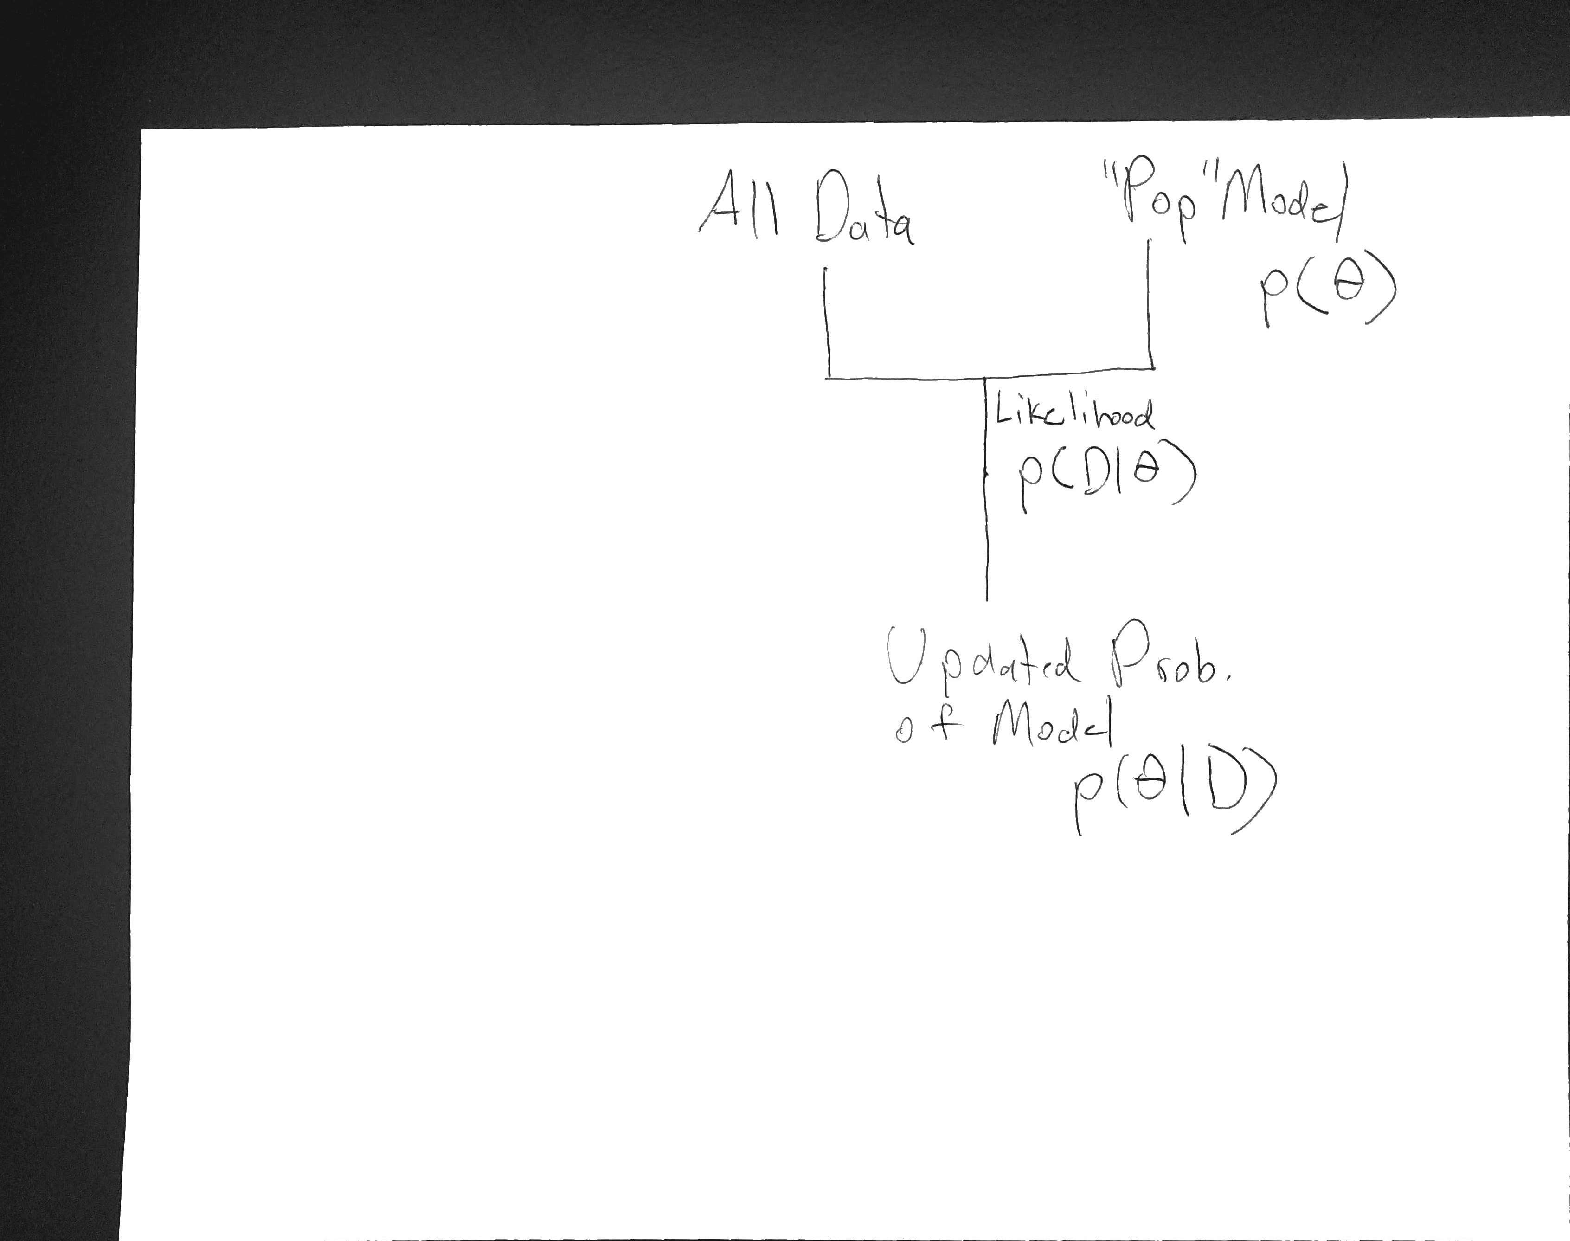
\includegraphics[height=.85\textheight]{e2e_flow.pdf}
\end{frame}

%----------- slide --------------------------------------------------%
\begin{frame}[t]
  \frametitle{A simulation demonstrating failure of SPDs}
    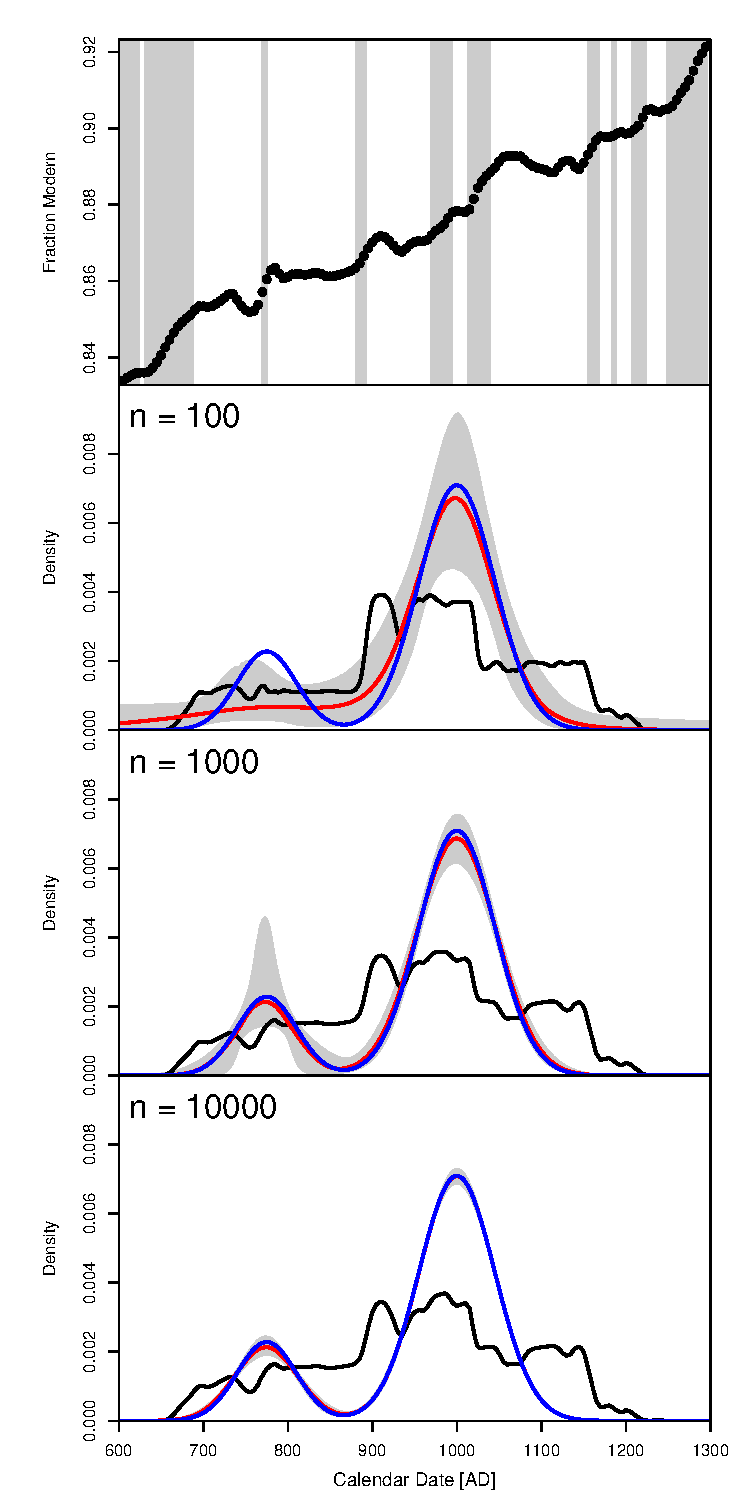
\includegraphics[height=.85\textheight]{Fig1_sim_inference.pdf}
\end{frame}

%----------- slide --------------------------------------------------%
\begin{frame}[t]
    \frametitle{Bayesian Inference}
   
    \begin{columns}[c]
        \column{.333\textwidth}
            \begin{flushright}
                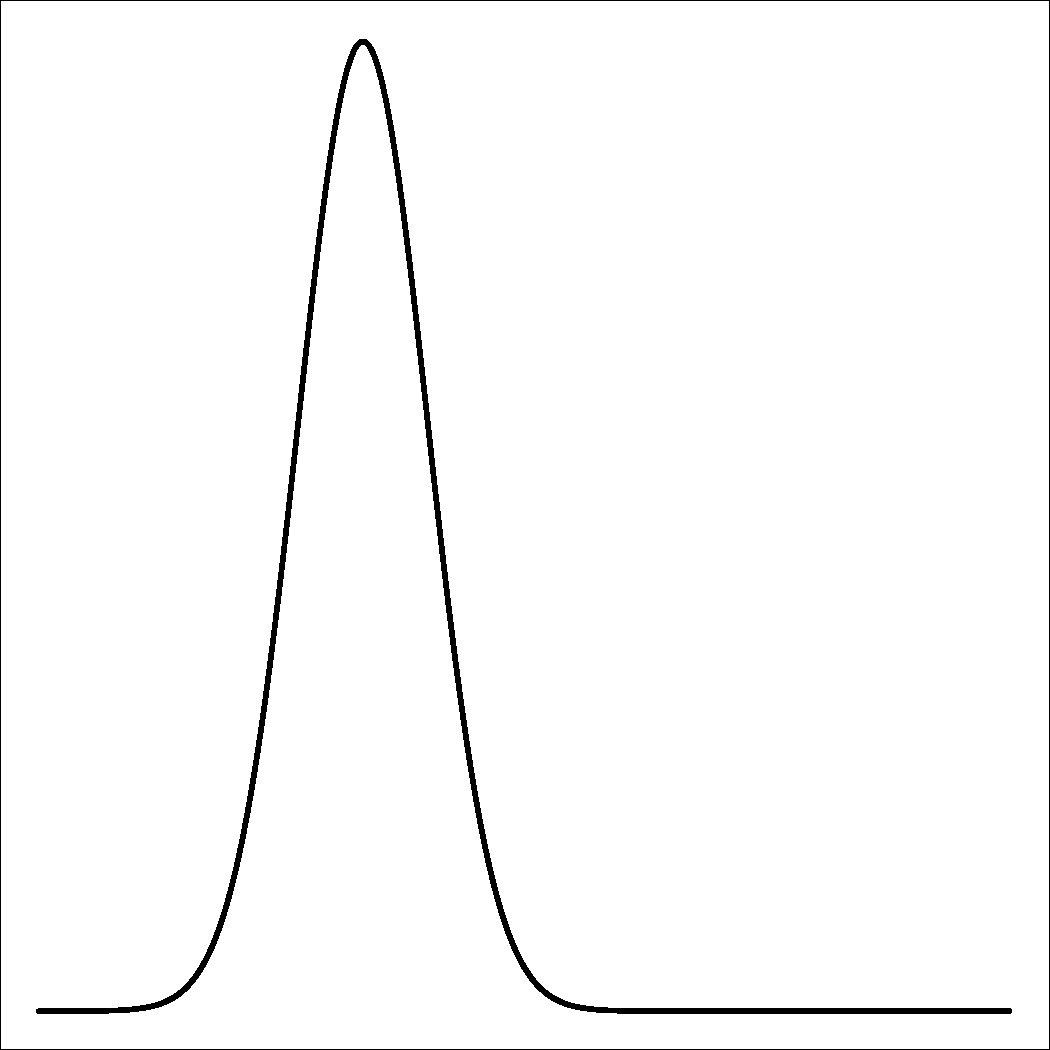
\includegraphics[width=1\textwidth]{bayesian_update_illustration_th1.pdf}
            \end{flushright}
        \column{.333\textwidth}
            \begin{flushright}
                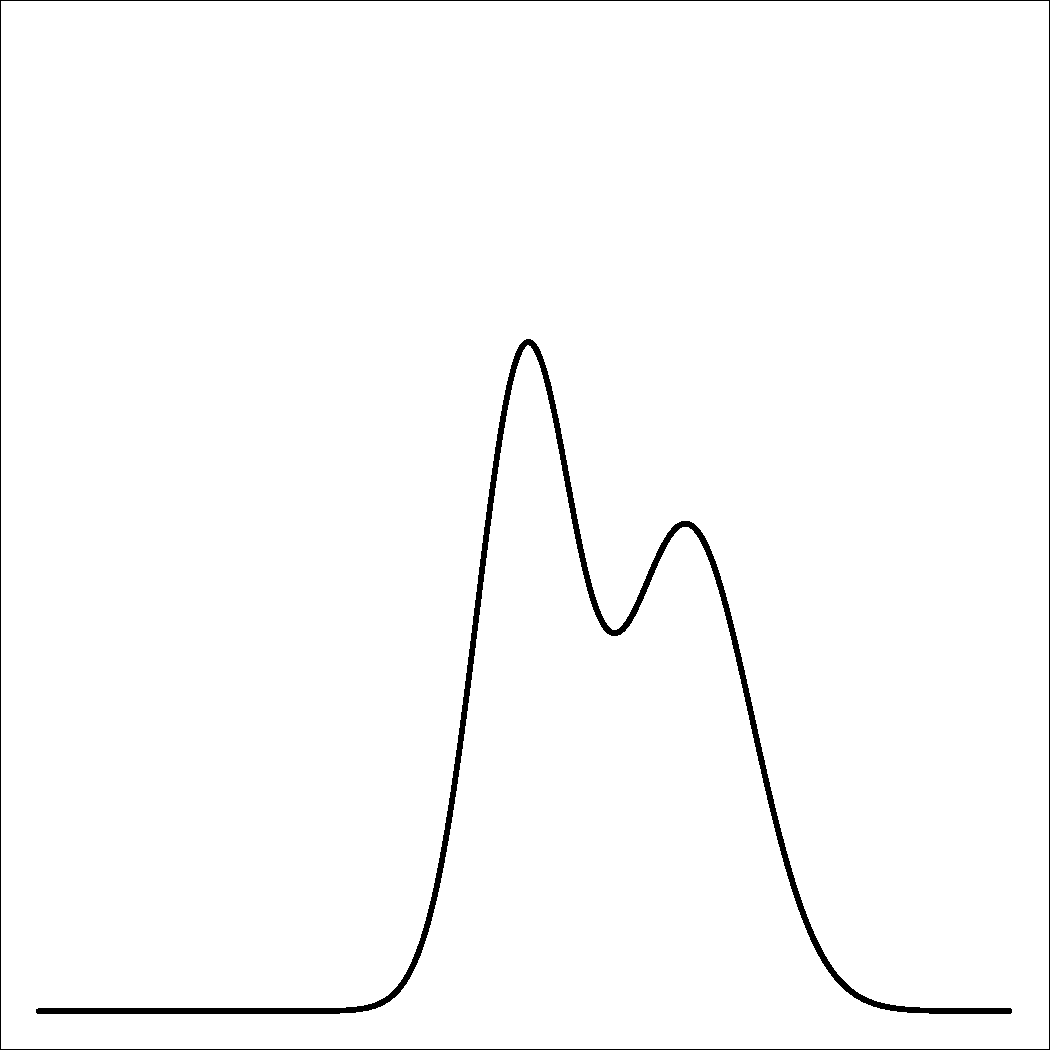
\includegraphics[width=1\textwidth]{bayesian_update_illustration_th2.pdf}
            \end{flushright}
        \column{.333\textwidth}
            \begin{flushright}
                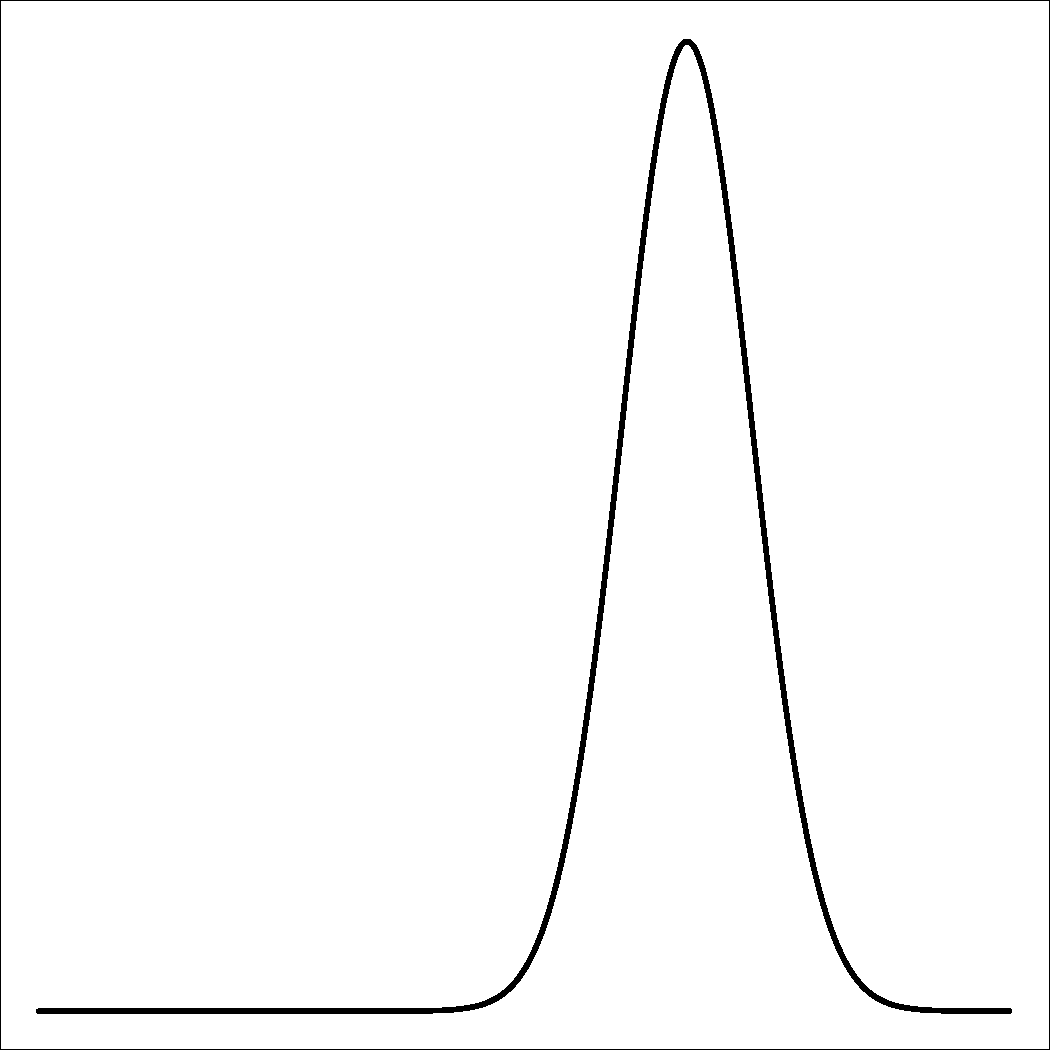
\includegraphics[width=1\textwidth]{bayesian_update_illustration_th3.pdf}
            \end{flushright}
    \end{columns}
\end{frame}

%----------- slide --------------------------------------------------%
\begin{frame}[t]
    \frametitle{Bayesian Inference}
    \begin{columns}[c]
        \column{.333\textwidth}
            \begin{flushright}
                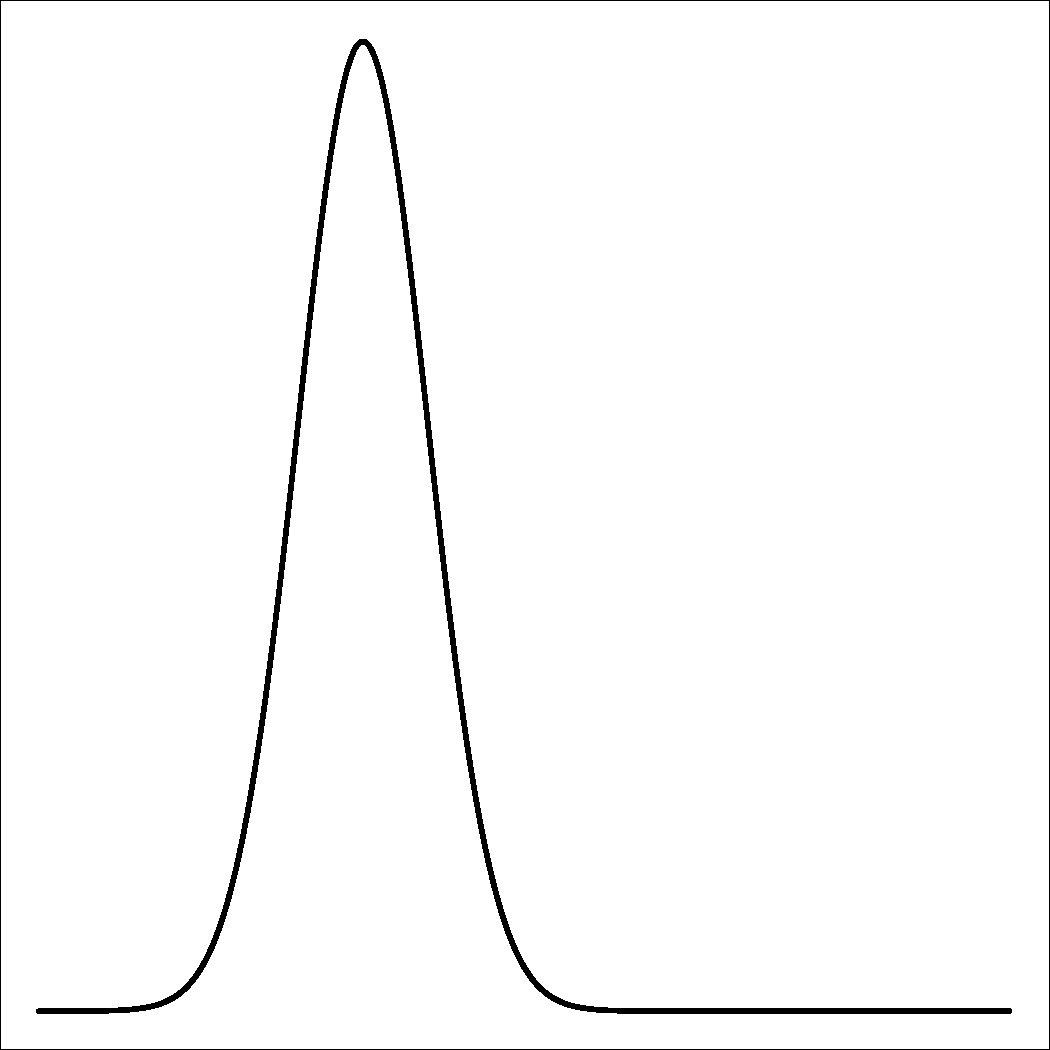
\includegraphics[width=1\textwidth]{bayesian_update_illustration_th1.pdf}\\
                \vspace{10pt}
                \Large Prior \hfill $0.40$\\
            \end{flushright}
        \column{.333\textwidth}
            \begin{flushright}
                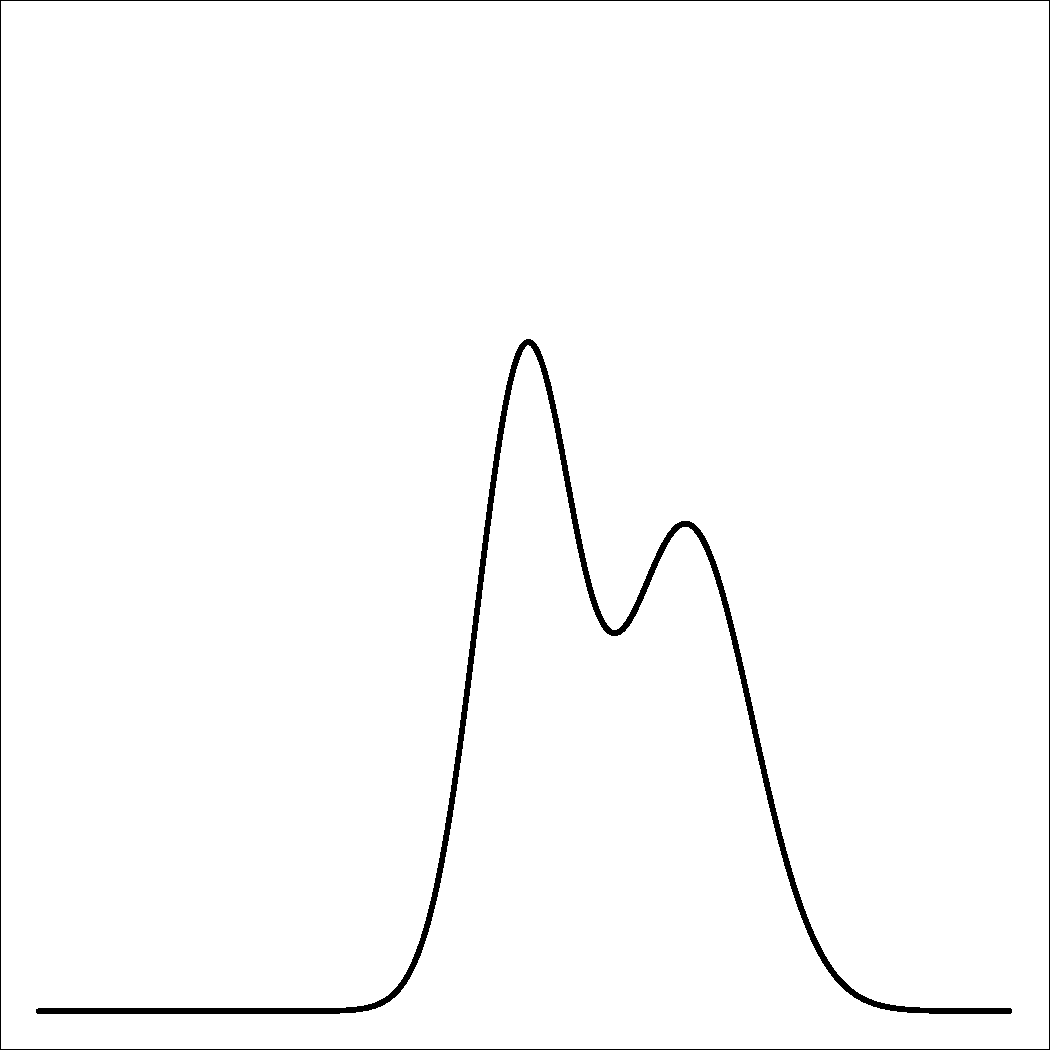
\includegraphics[width=1\textwidth]{bayesian_update_illustration_th2.pdf}\\
                \vspace{10pt}
                \Large $0.20$\\
            \end{flushright}
        \column{.333\textwidth}
            \begin{flushright}
                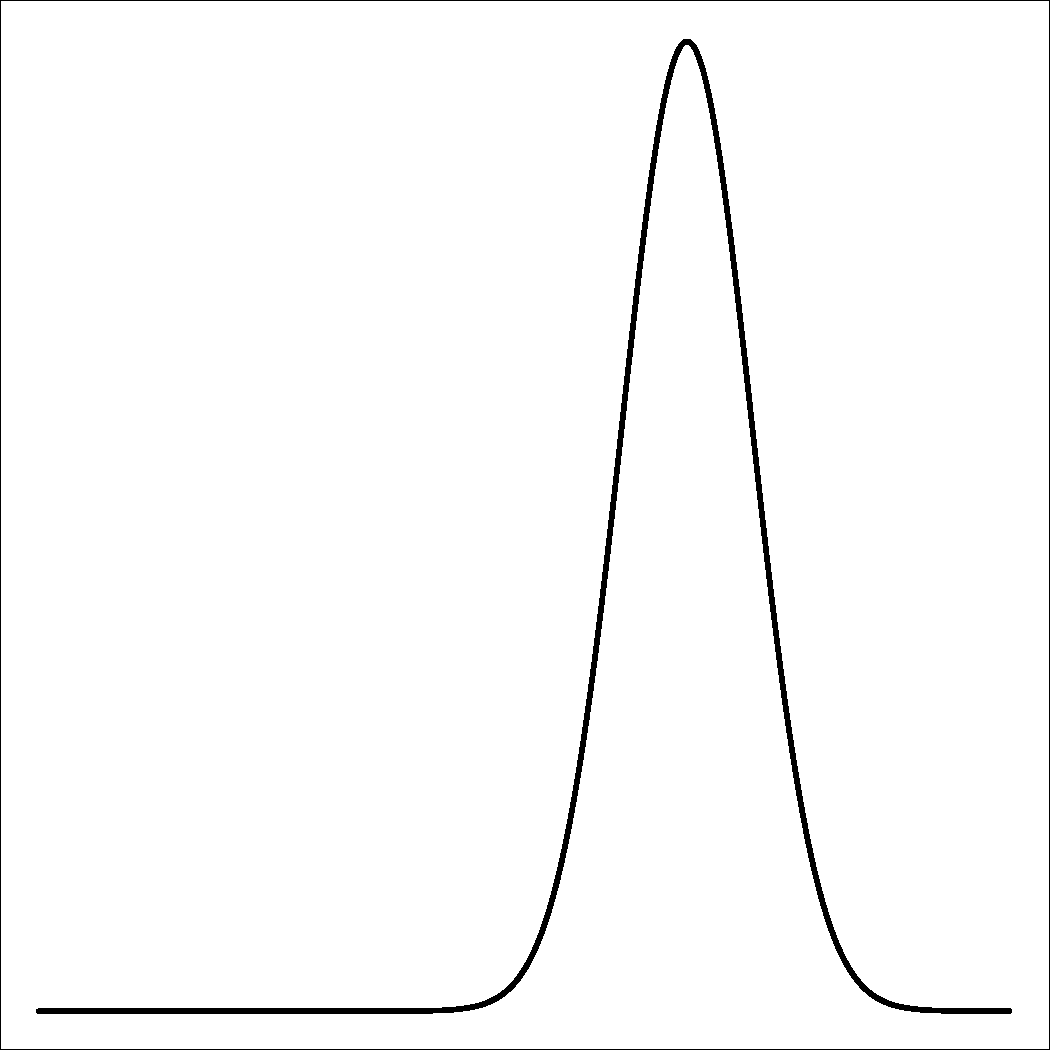
\includegraphics[width=1\textwidth]{bayesian_update_illustration_th3.pdf}\\
                \vspace{10pt}
                \Large $0.4$\\
            \end{flushright}
    \end{columns}
\end{frame}

%----------- slide --------------------------------------------------%
\begin{frame}[t]
    \frametitle{Bayesian Inference}
    \begin{columns}[c]
        \column{.333\textwidth}
            \begin{flushright}
                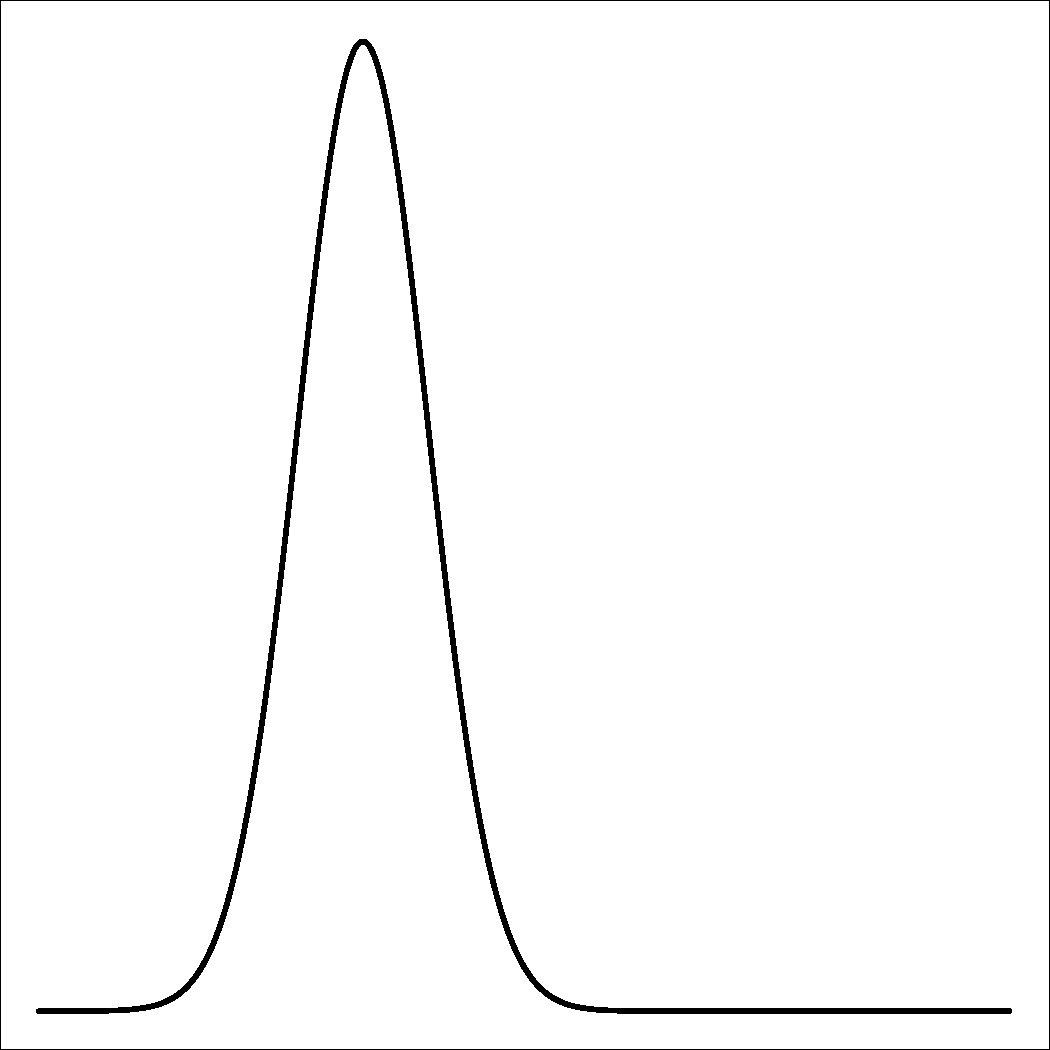
\includegraphics[width=1\textwidth]{bayesian_update_illustration_th1.pdf}\\
                \vspace{10pt}
                \Large Prior \hfill $0.40$\\
                \vspace{20pt}
                \Large Likelihood \hfill $0.02$\\
            \end{flushright}
        \column{.333\textwidth}
            \begin{flushright}
                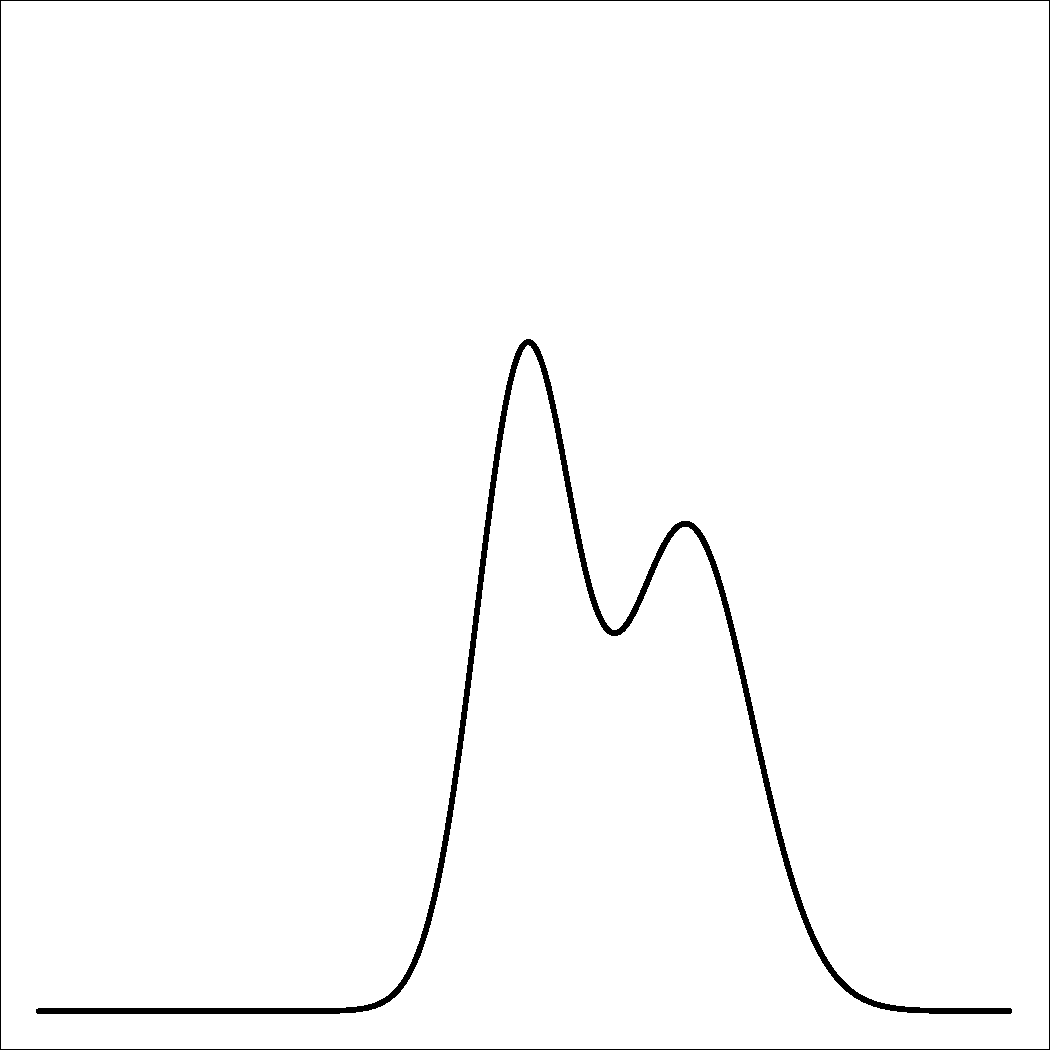
\includegraphics[width=1\textwidth]{bayesian_update_illustration_th2.pdf}\\
                \vspace{10pt}
                \Large $0.20$\\
                \vspace{20pt}
                \Large $1.00$\\
            \end{flushright}
        \column{.333\textwidth}
            \begin{flushright}
                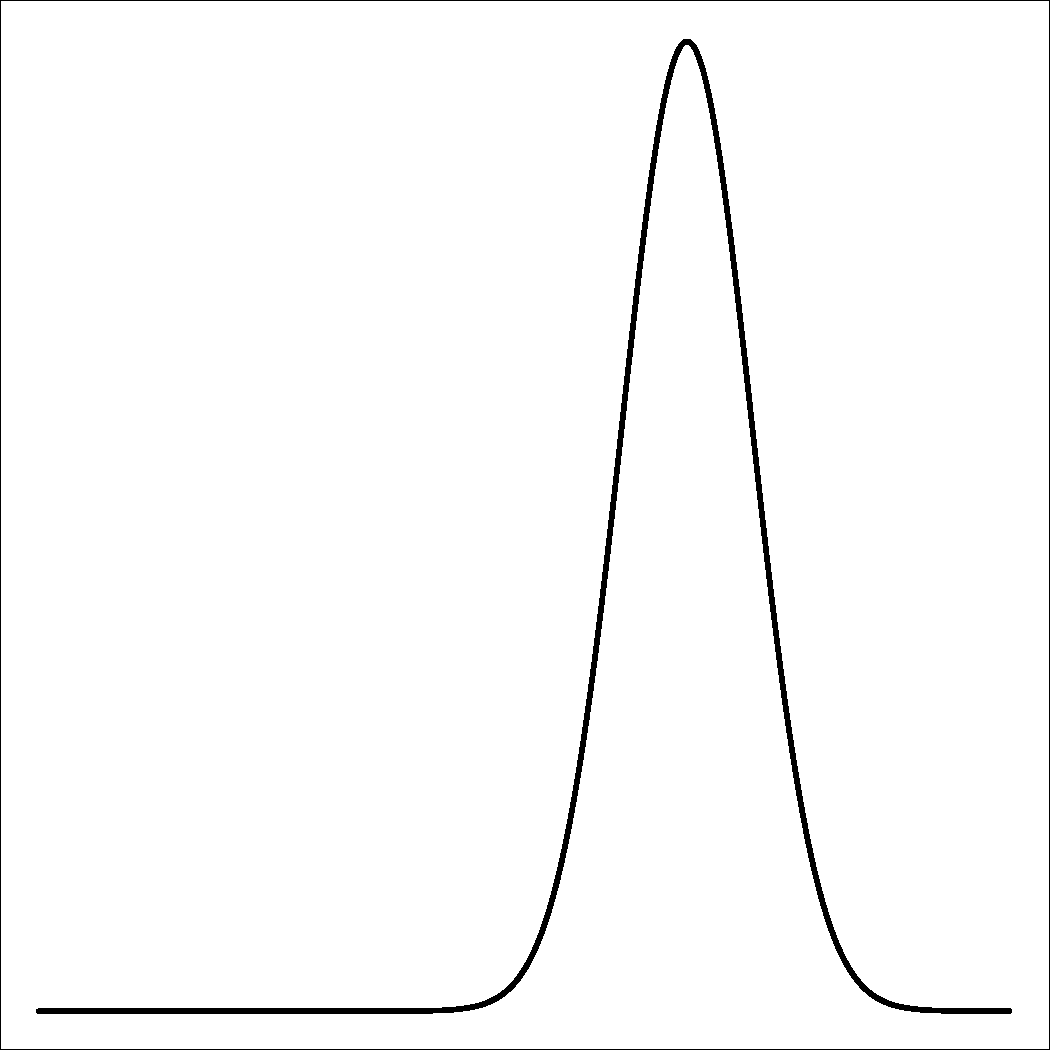
\includegraphics[width=1\textwidth]{bayesian_update_illustration_th3.pdf}\\
                \vspace{10pt}
                \Large $0.4$\\
                \vspace{20pt}
                \Large $0.04$\\
            \end{flushright}
    \end{columns}
\end{frame}

%----------- slide --------------------------------------------------%
\begin{frame}[t]
    \frametitle{Bayesian Inference}
    \begin{columns}[c]
        \column{.333\textwidth}
            \begin{flushright}
                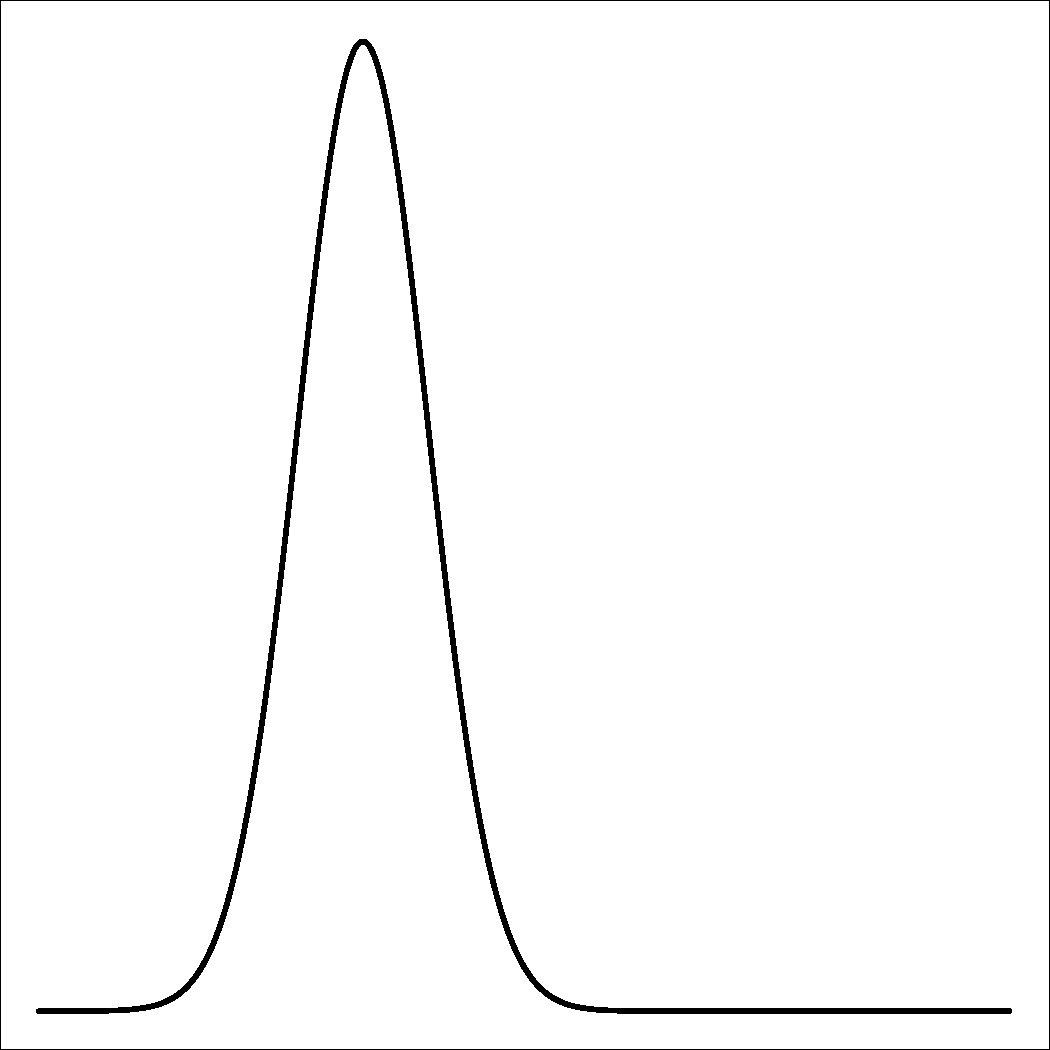
\includegraphics[width=1\textwidth]{bayesian_update_illustration_th1.pdf}\\
                \vspace{10pt}
                \Large Prior \hfill $0.40$\\
                \vspace{20pt}
                \Large Likelihood \hfill $0.02$\\
                \vspace{20pt}
                \Large Posterior \hfill $0.02$
            \end{flushright}
        \column{.333\textwidth}
            \begin{flushright}
                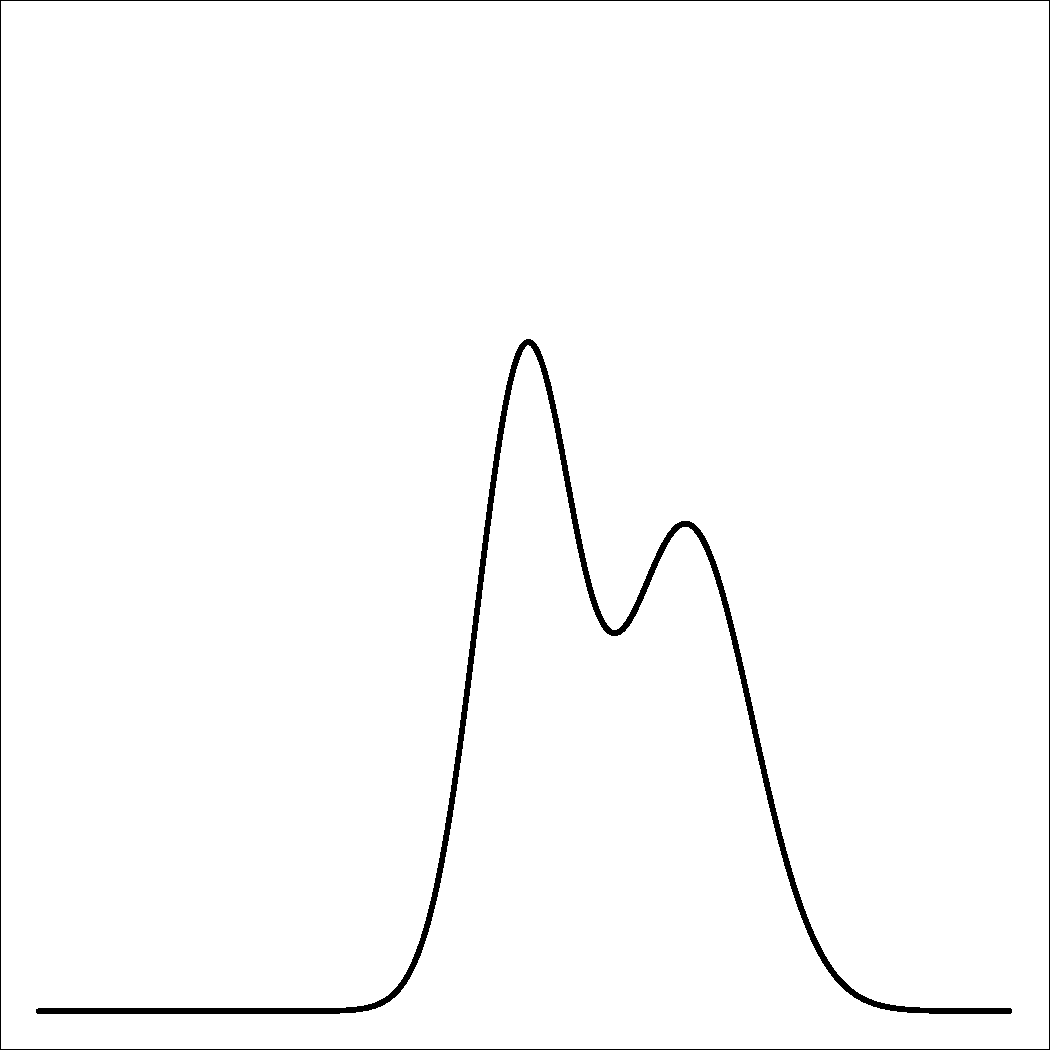
\includegraphics[width=1\textwidth]{bayesian_update_illustration_th2.pdf}\\
                \vspace{10pt}
                \Large $0.20$\\
                \vspace{20pt}
                \Large $1.00$\\
                \vspace{20pt}
                \Large $0.94$
            \end{flushright}
        \column{.333\textwidth}
            \begin{flushright}
                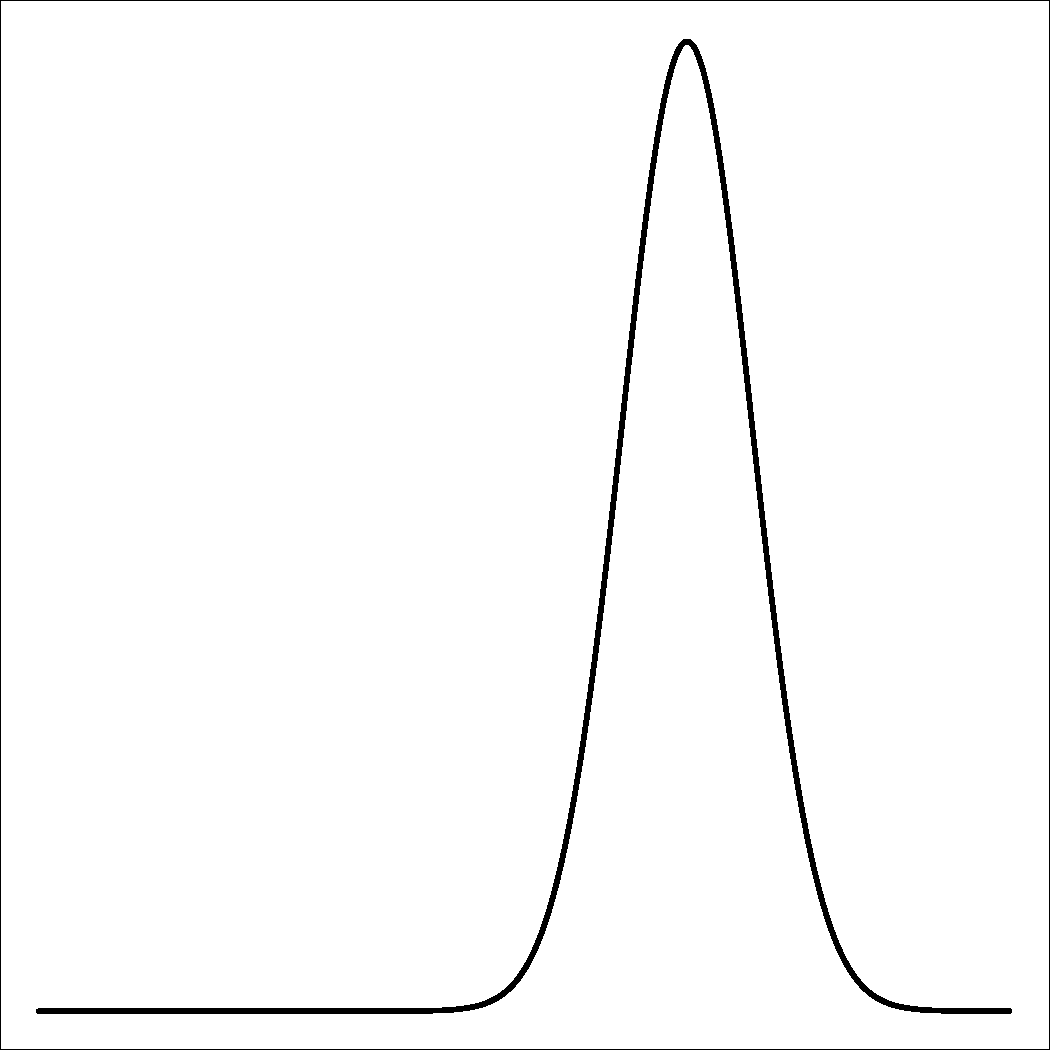
\includegraphics[width=1\textwidth]{bayesian_update_illustration_th3.pdf}\\
                \vspace{10pt}
                \Large $0.4$\\
                \vspace{20pt}
                \Large $0.04$\\
                \vspace{20pt}
                \Large $0.04$
            \end{flushright}
    \end{columns}
\end{frame}

%----------- slide --------------------------------------------------%
\begin{frame}[t]
    \frametitle{Bayesian Inference}
    \begin{columns}[c]
        \column{.333\textwidth}
            \begin{flushright}
                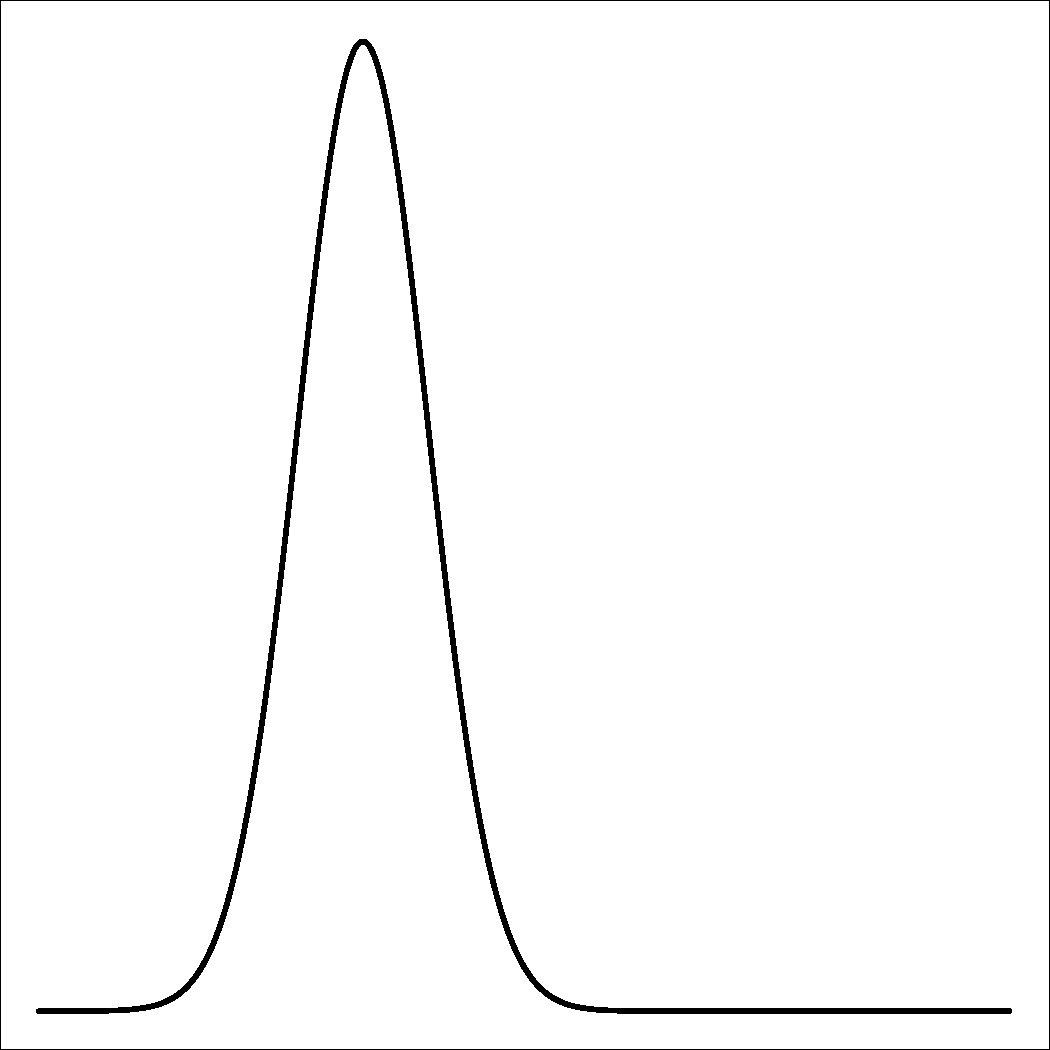
\includegraphics[width=1\textwidth]{bayesian_update_illustration_th1.pdf}\\
                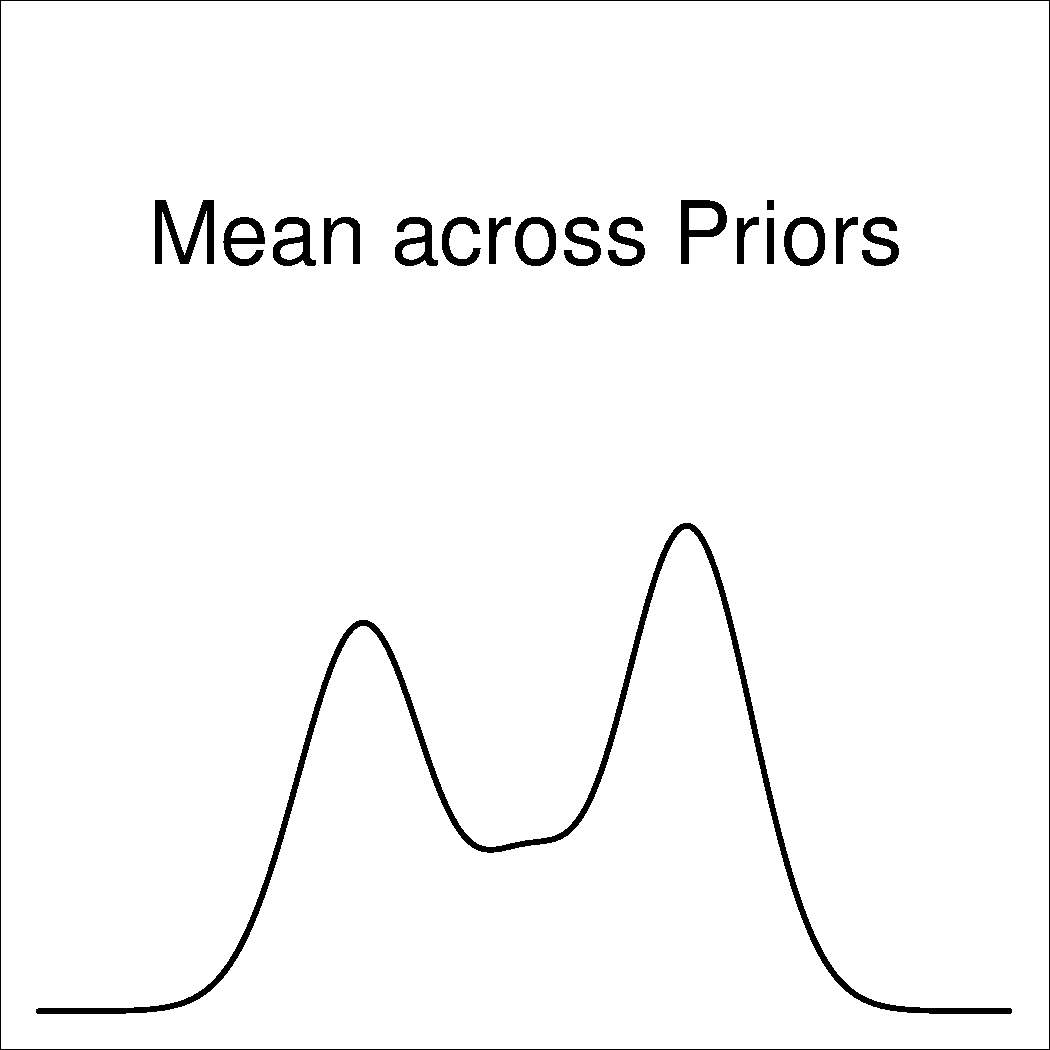
\includegraphics[width=1\textwidth]{bayesian_update_illustration_prior.pdf}\\
            \end{flushright}
        \column{.333\textwidth}
            \begin{flushright}
                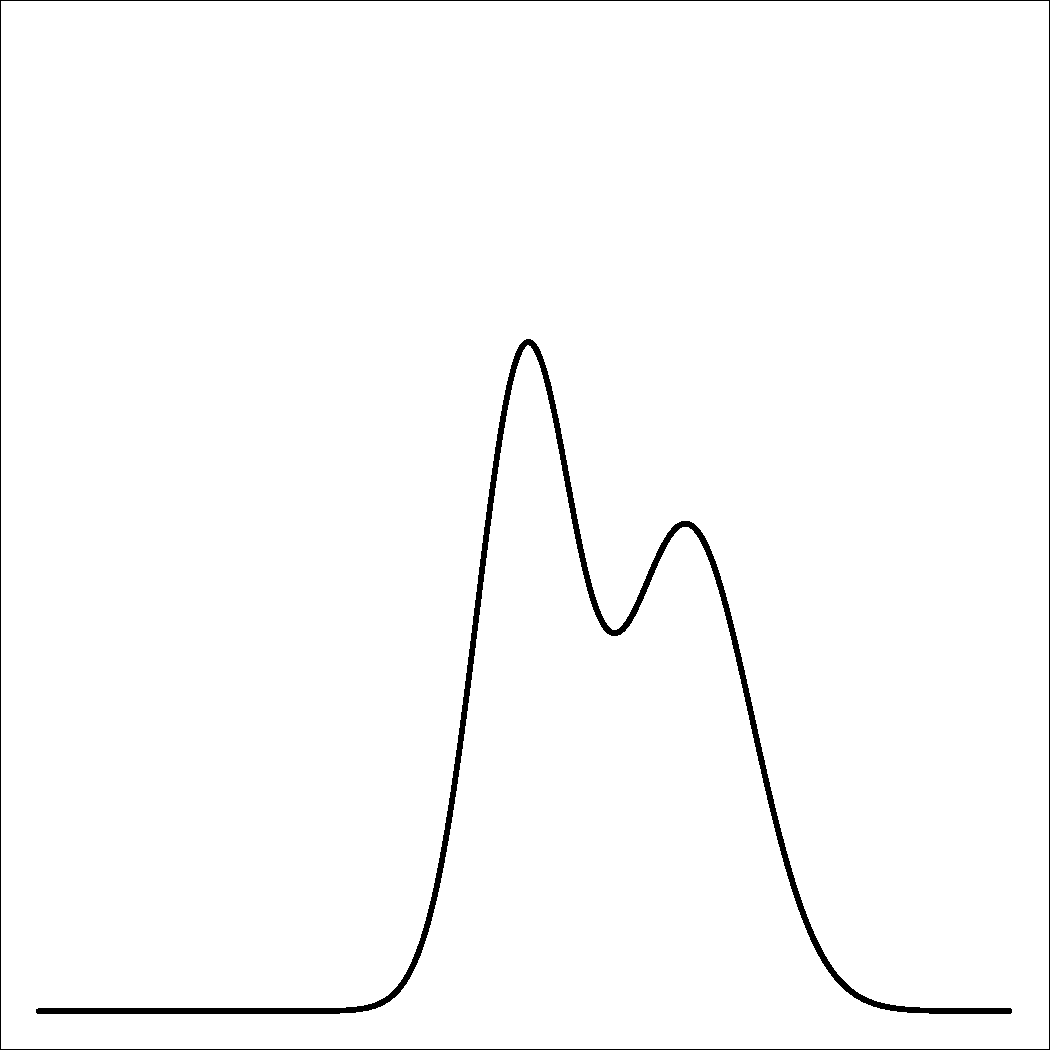
\includegraphics[width=1\textwidth]{bayesian_update_illustration_th2.pdf}\\
                
\includegraphics[width=1\textwidth]{bayesian_update_illustration_blank.pdf}\\
            \end{flushright}
        \column{.333\textwidth}
            \begin{flushright}
                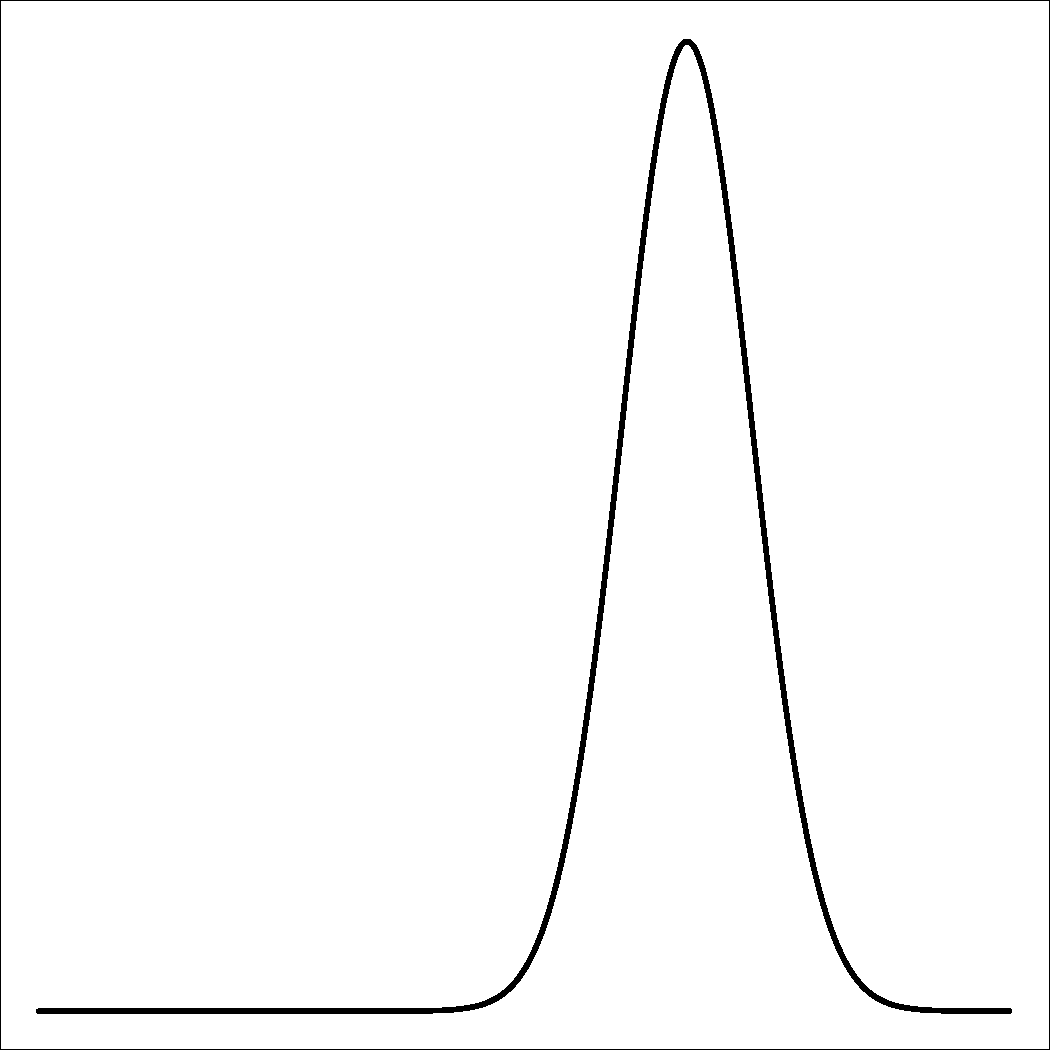
\includegraphics[width=1\textwidth]{bayesian_update_illustration_th3.pdf}\\
                
\includegraphics[width=1\textwidth]{bayesian_update_illustration_blank.pdf}\\
            \end{flushright}
    \end{columns}
\end{frame}

%----------- slide --------------------------------------------------%
\begin{frame}[t]
    \frametitle{Bayesian Inference}
    \begin{columns}[c]
        \column{.333\textwidth}
            \begin{flushright}
                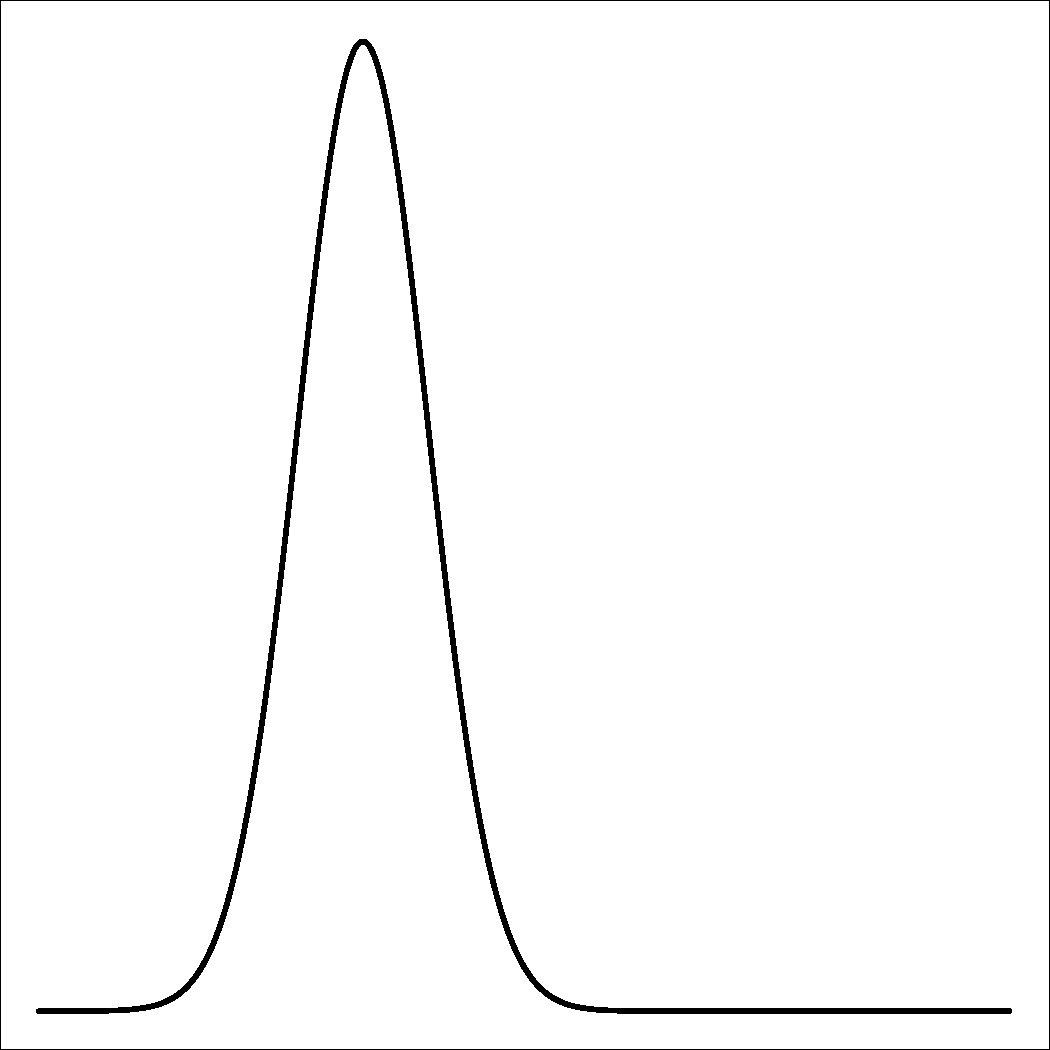
\includegraphics[width=1\textwidth]{bayesian_update_illustration_th1.pdf}\\
                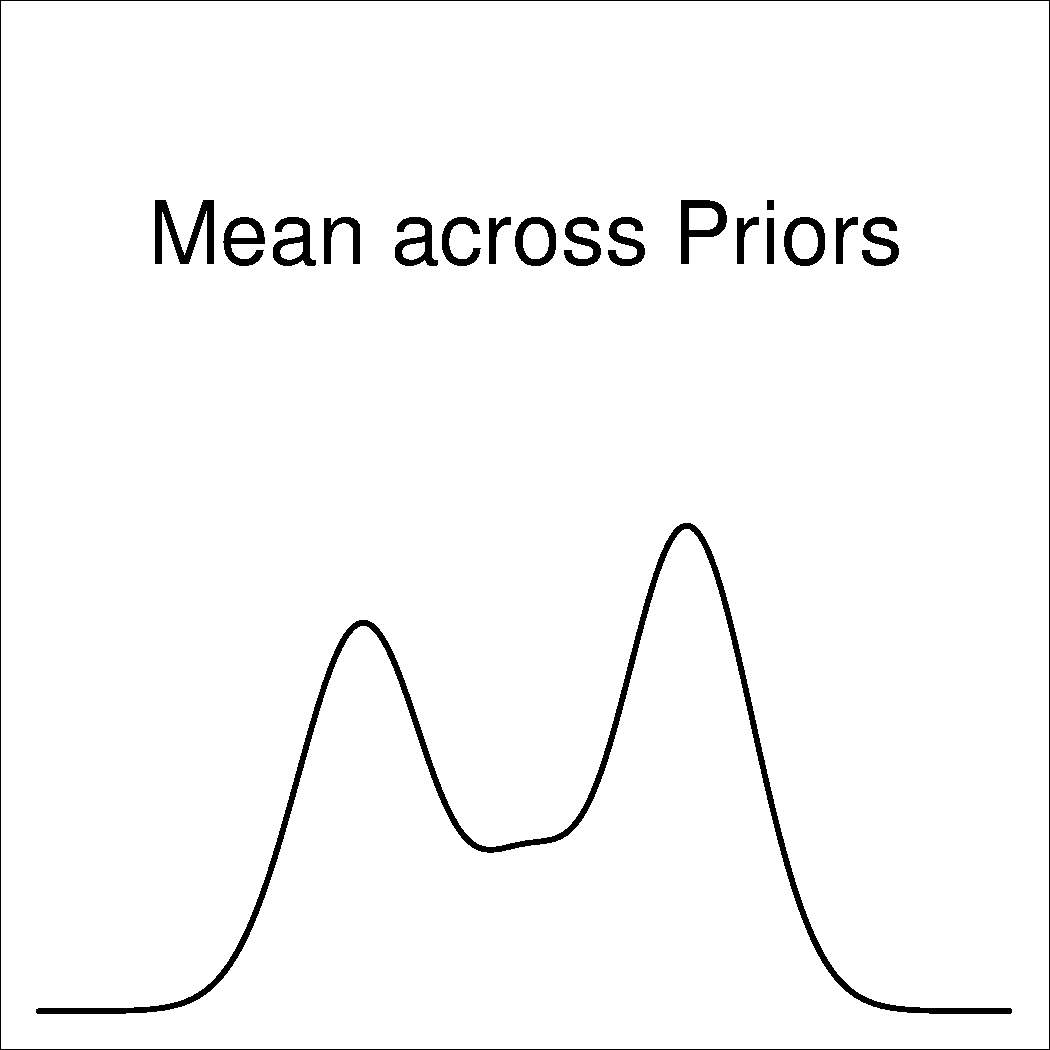
\includegraphics[width=1\textwidth]{bayesian_update_illustration_prior.pdf}\\
            \end{flushright}
        \column{.333\textwidth}
            \begin{flushright}
                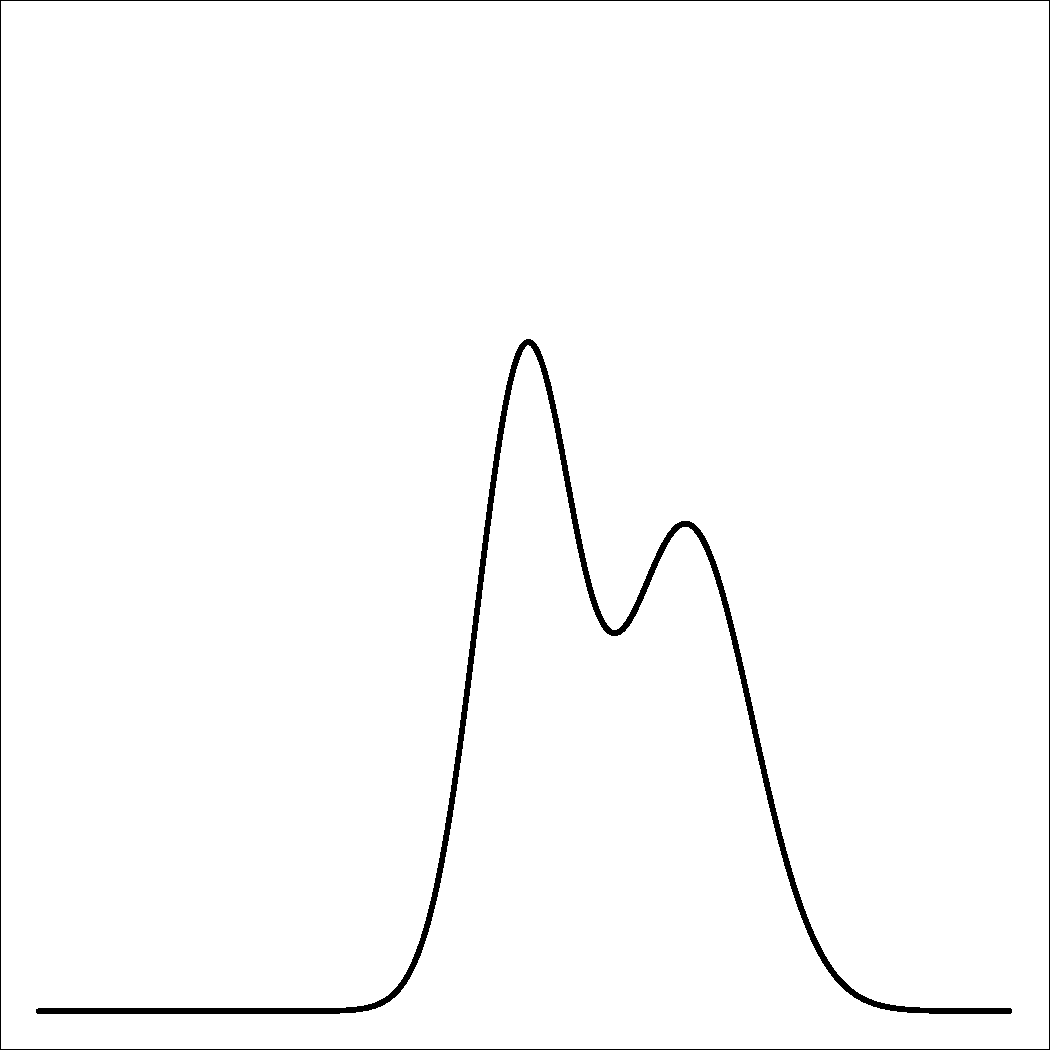
\includegraphics[width=1\textwidth]{bayesian_update_illustration_th2.pdf}\\
                
\includegraphics[width=1\textwidth]{bayesian_update_illustration_blank.pdf}\\
            \end{flushright}
        \column{.333\textwidth}
            \begin{flushright}
                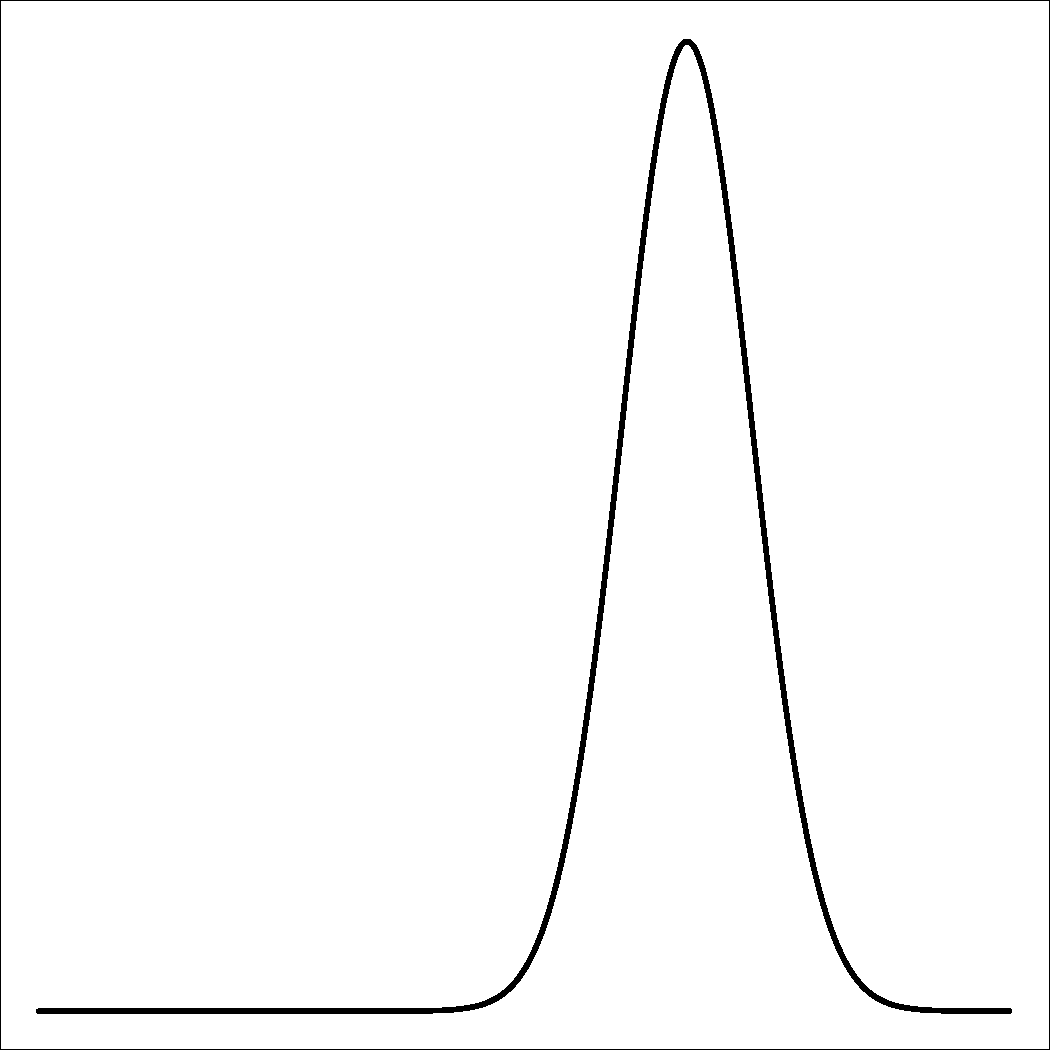
\includegraphics[width=1\textwidth]{bayesian_update_illustration_th3.pdf}\\
                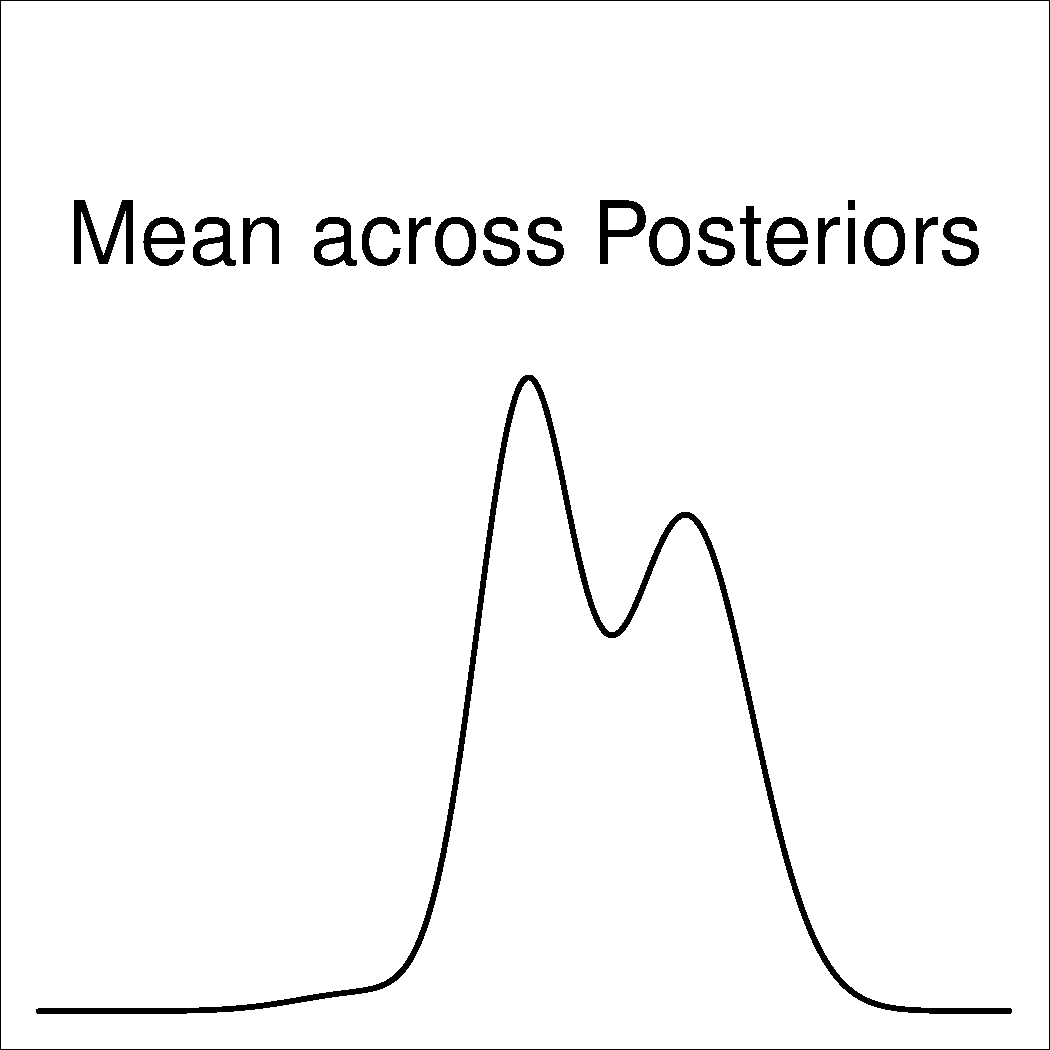
\includegraphics[width=1\textwidth]{bayesian_update_illustration_posterior.pdf}\\
            \end{flushright}
    \end{columns}
\end{frame}

%----------- slide --------------------------------------------------%
\begin{frame}
  \frametitle{Bayesian Inference}
  \begin{center}
	\begin{equation*}
          p(\greekbf{\theta}|\mathbf{D},\greekbf{\alpha}) = \frac{p(\mathbf{D}|\greekbf{\theta}) \, p(\greekbf{\theta}|\greekbf{\alpha})}{p(\mathbf{D}|\greekbf{\alpha})}
        \end{equation*}
  \end{center}

  \pause
  \begin{center}
          \begin{equation*}
            \begin{array}{lll}
	      \greekbf{\alpha} & := & \mbox{Hyperparameter specifying priors}\\
                               &    &\\
              \greekbf{\theta} & := & \mbox{Parameter for demographic models}\\
	      \pause
                               &    &\\
              \mathbf{D}       & := & \mbox{Data}\\
                               &    &\\
            \end{array}
          \end{equation*}
  \end{center}
\end{frame}

%----------- slide --------------------------------------------------%
\begin{frame}
  \frametitle{Bayesian Inference [Gibbs, MCMC, etc.]}
  \Large
  What if $p(\greekbf{\theta}|\mathbf{D},\greekbf{\alpha})$ is hard to calculate?\\
  \pause
  \vspace{.75cm}
  Sample from the posterior distribution using well-established techniques yielding $\greekbf{\theta}_n$\\
  \pause
  \vspace{.75cm}
  $<f> = \frac{1}{N} \, \sum_{n=1}^{N} f(\greekbf{\theta_n})$\\
\end{frame}

%----------- slide --------------------------------------------------%
\begin{frame}[t]
  \frametitle{Back to simulation}
    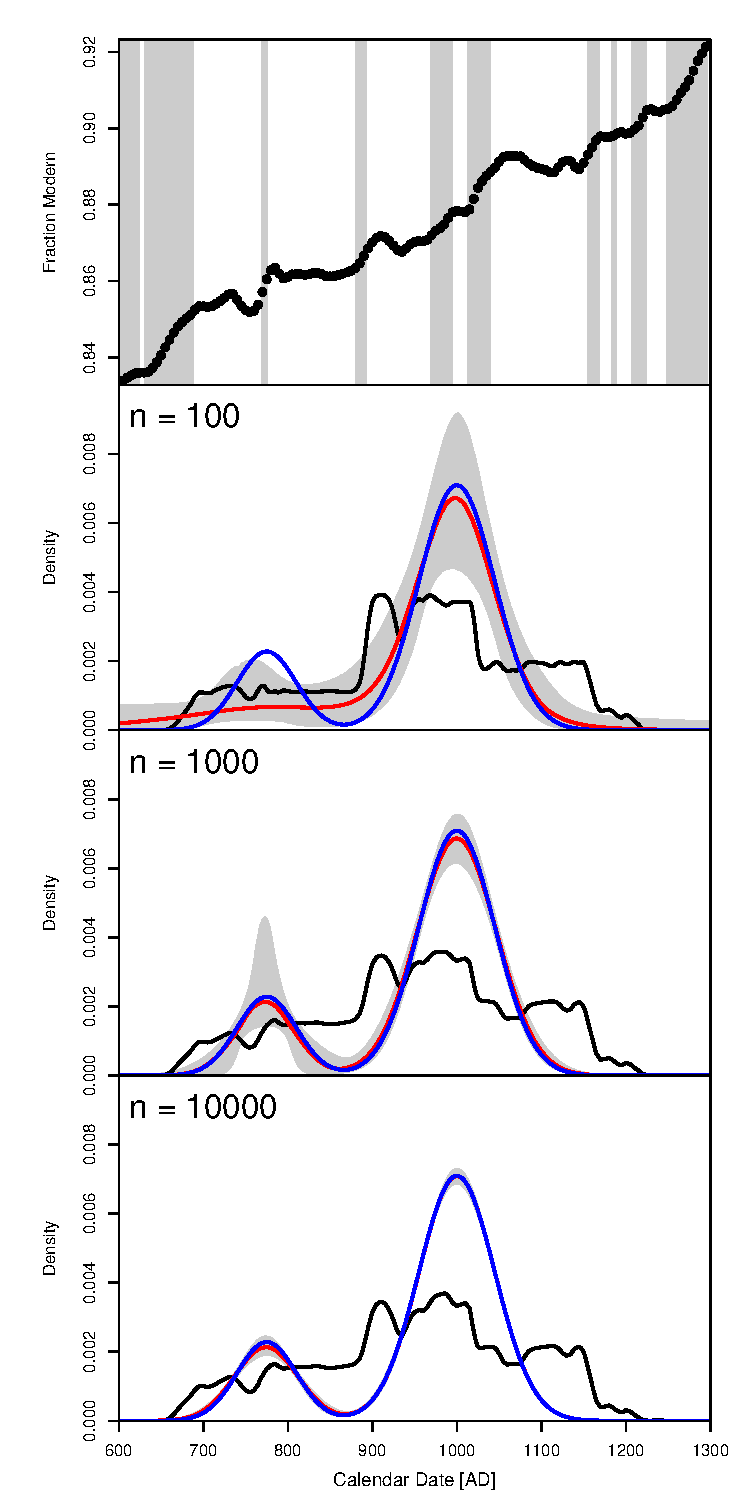
\includegraphics[height=.85\textheight]{Fig1_sim_inference.pdf}
\end{frame}

%----------- slide --------------------------------------------------%
\begin{frame}[t]
  \frametitle{Statistical Identifiability}
\end{frame}

%----------- slide --------------------------------------------------%
\begin{frame}[t]
  \frametitle{Maya Reconstructions}
    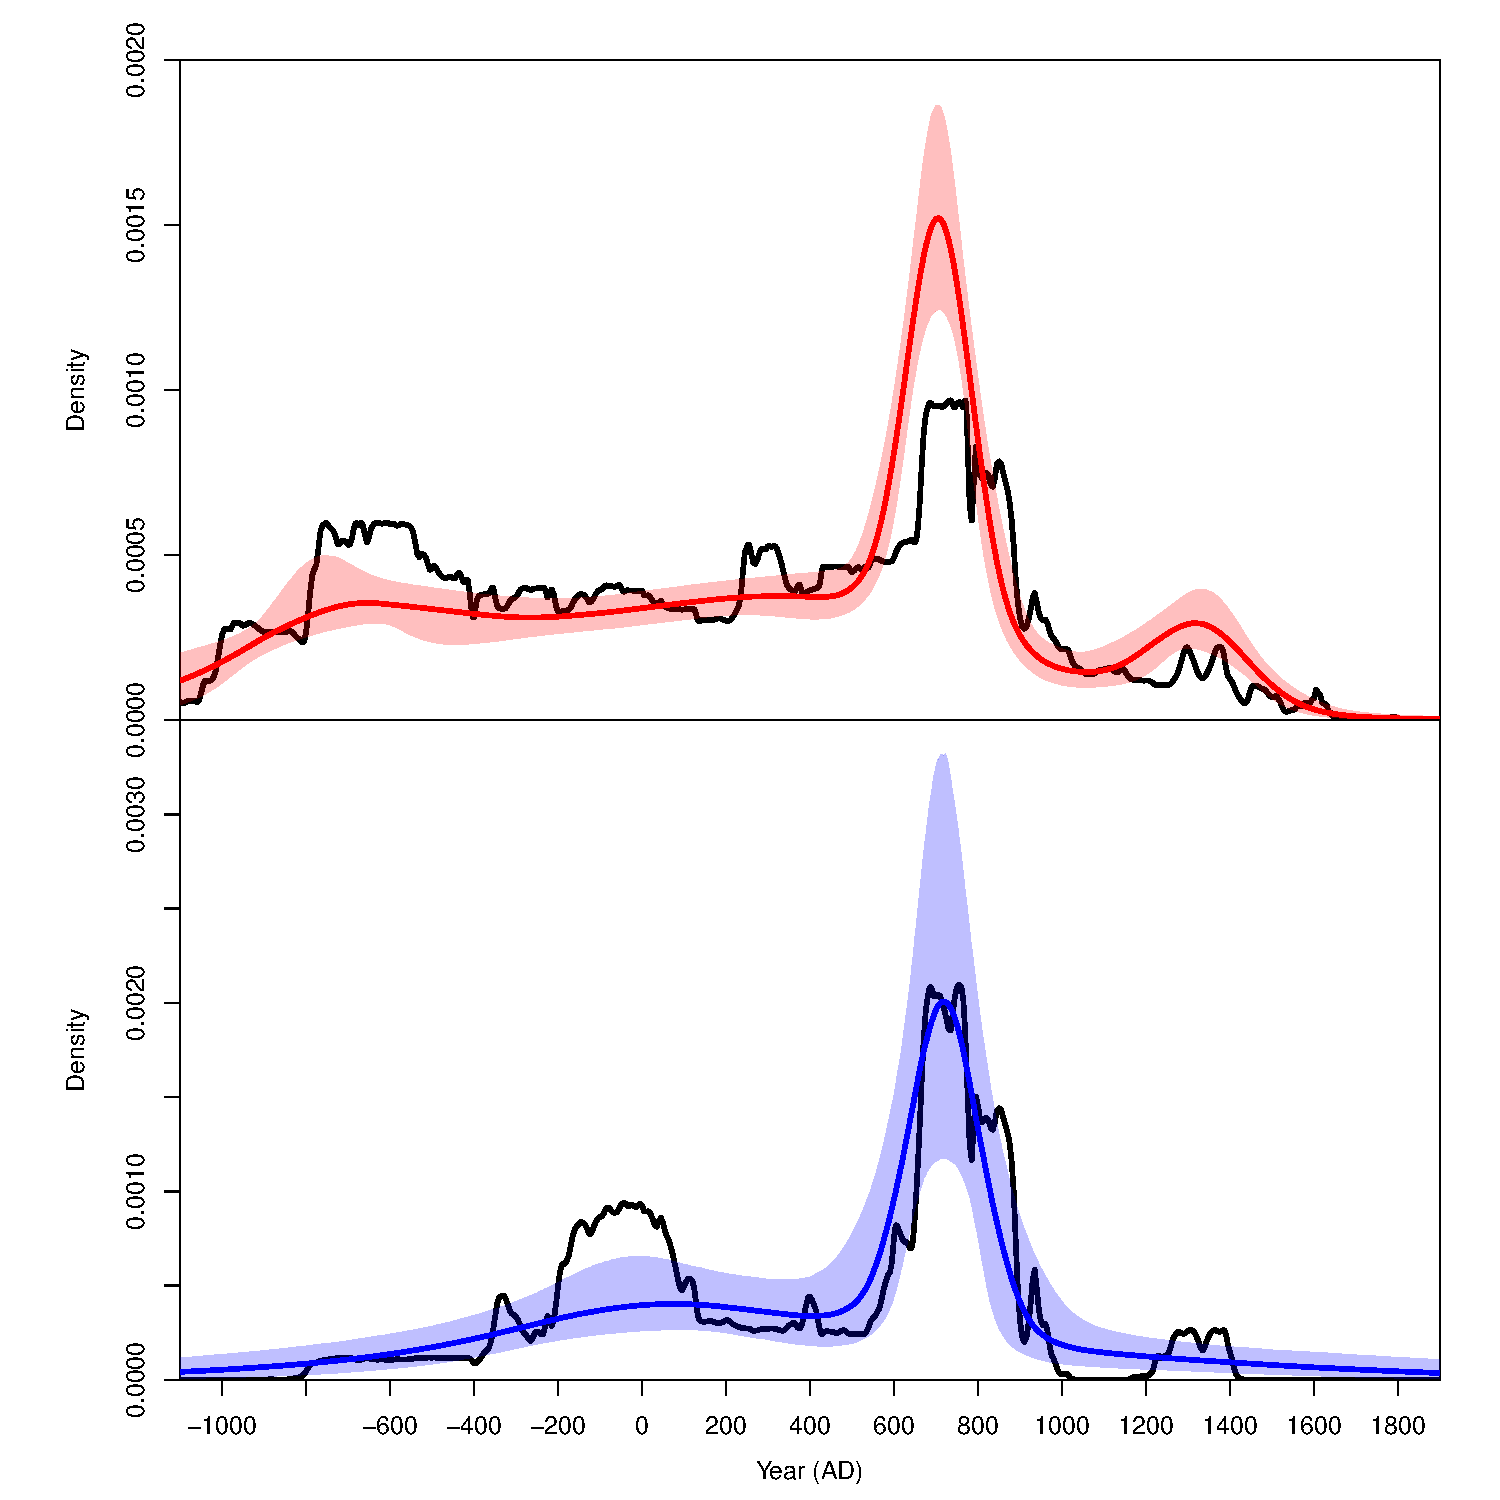
\includegraphics[height=.85\textheight]{Fig2_maya_inference_K10.pdf}
\end{frame}

%----------- slide --------------------------------------------------%
\begin{frame}[t]
  \frametitle{Maya Reconstructions}
    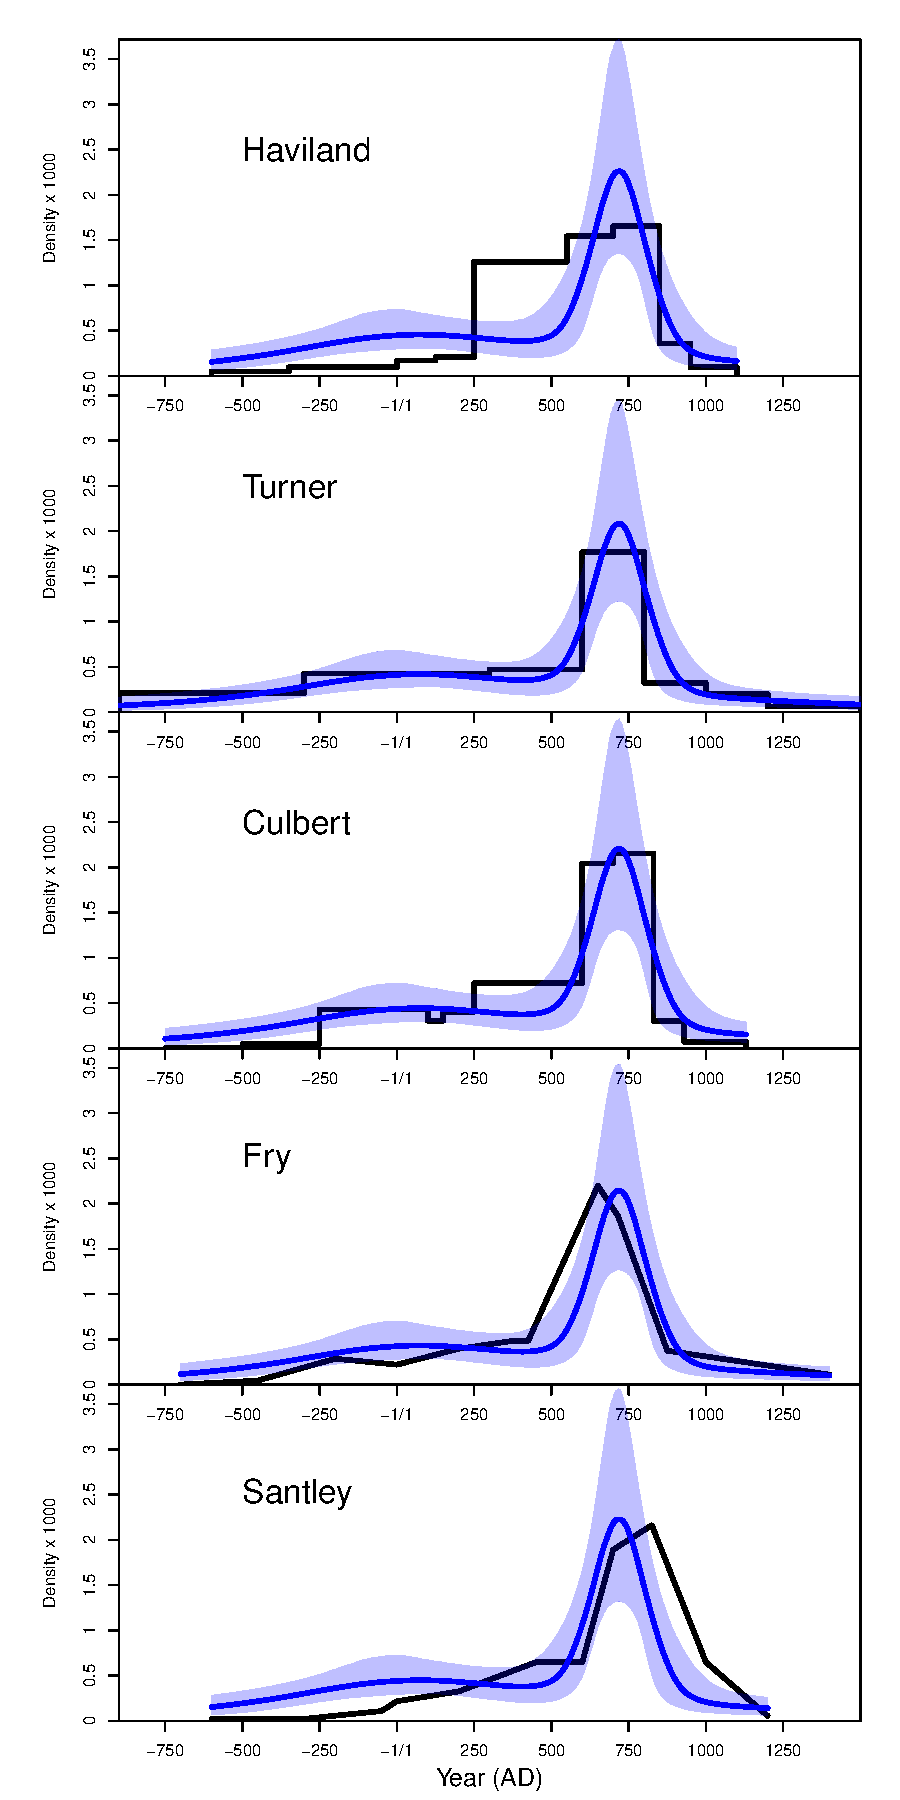
\includegraphics[height=.85\textheight]{Fig3_tikal_prev_expert_comparison.pdf}
\end{frame}

%----------- slide --------------------------------------------------%
\begin{frame}[t]
  \frametitle{Maya Reconstructions}
    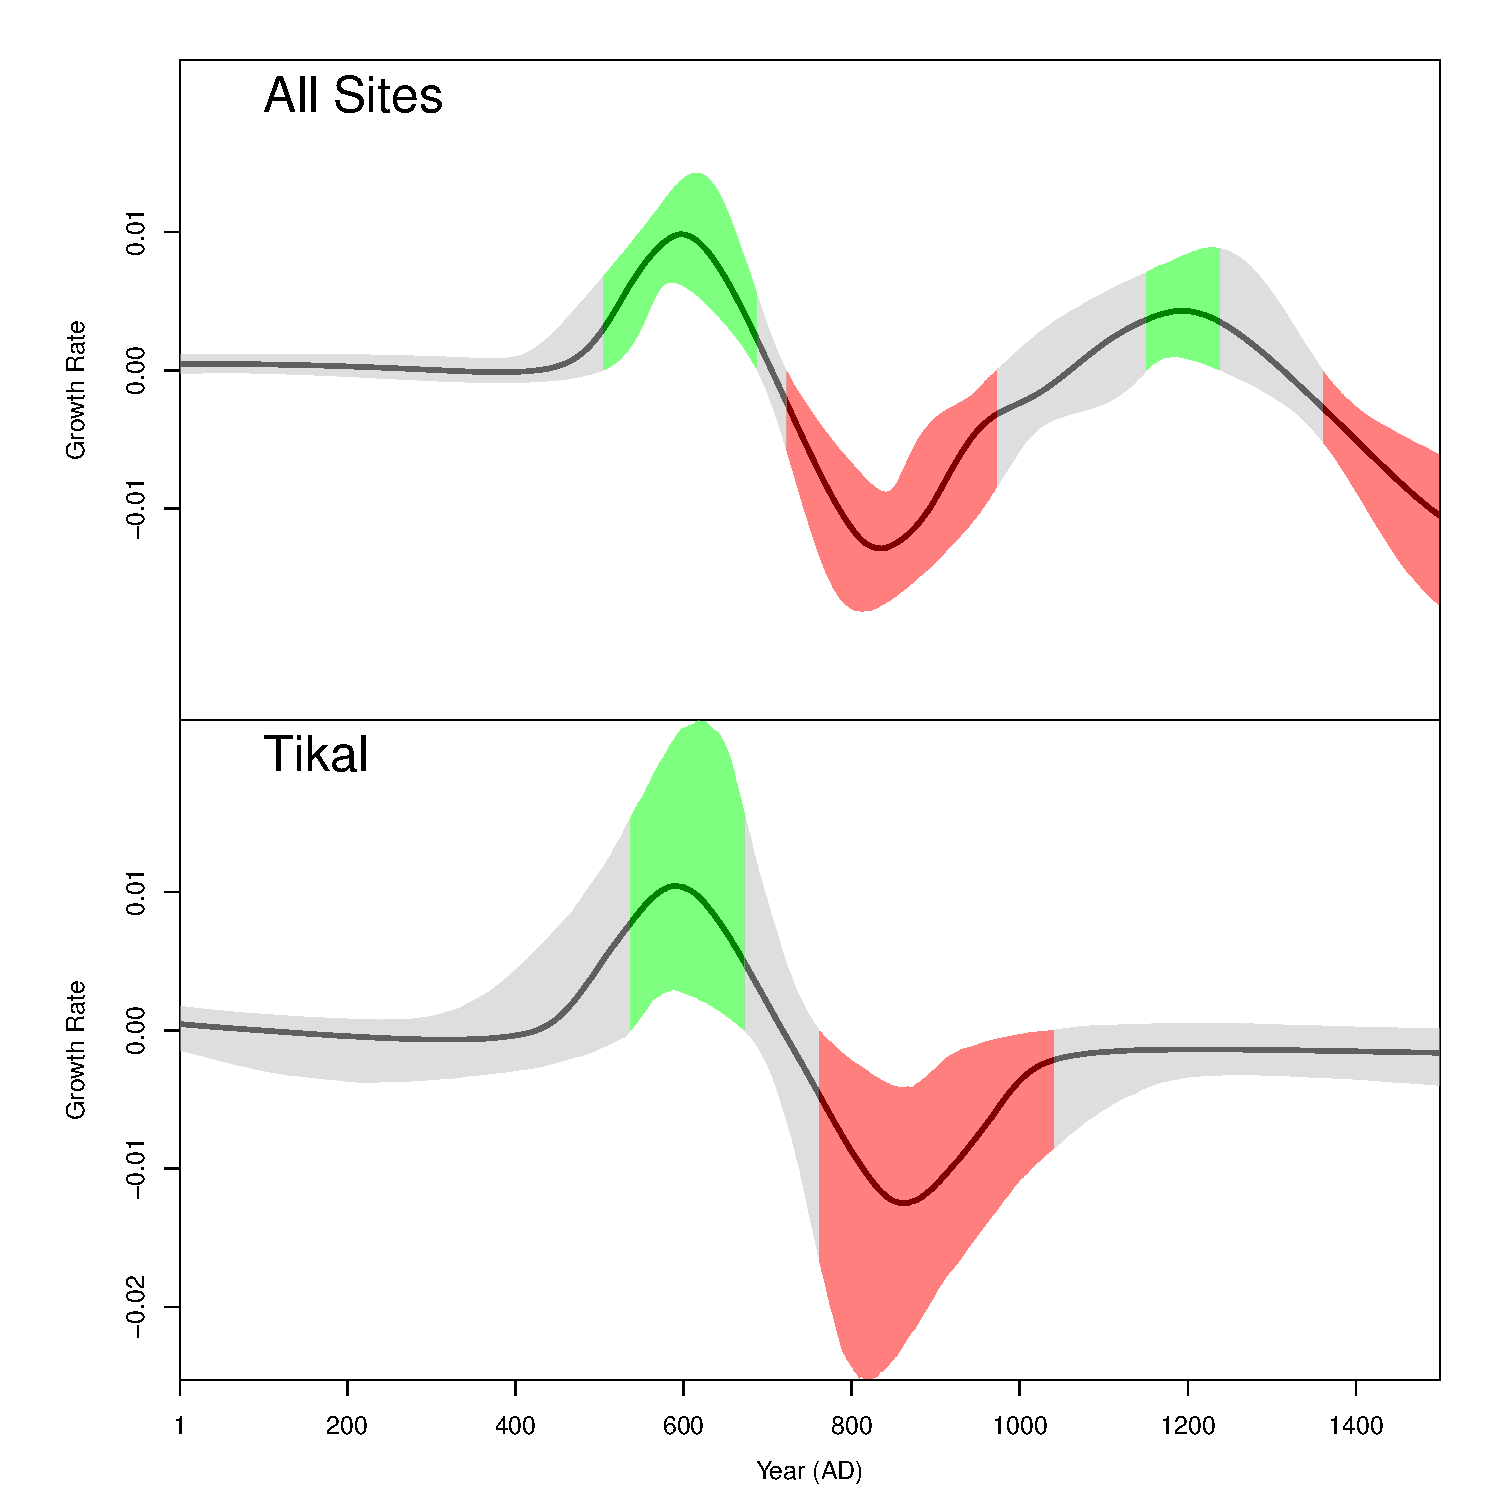
\includegraphics[height=.85\textheight]{Fig4_maya_inference_rate_K10.pdf}
\end{frame}

%----------- slide --------------------------------------------------%
\begin{frame}[t]
  \frametitle{Maya Reconstructions}
    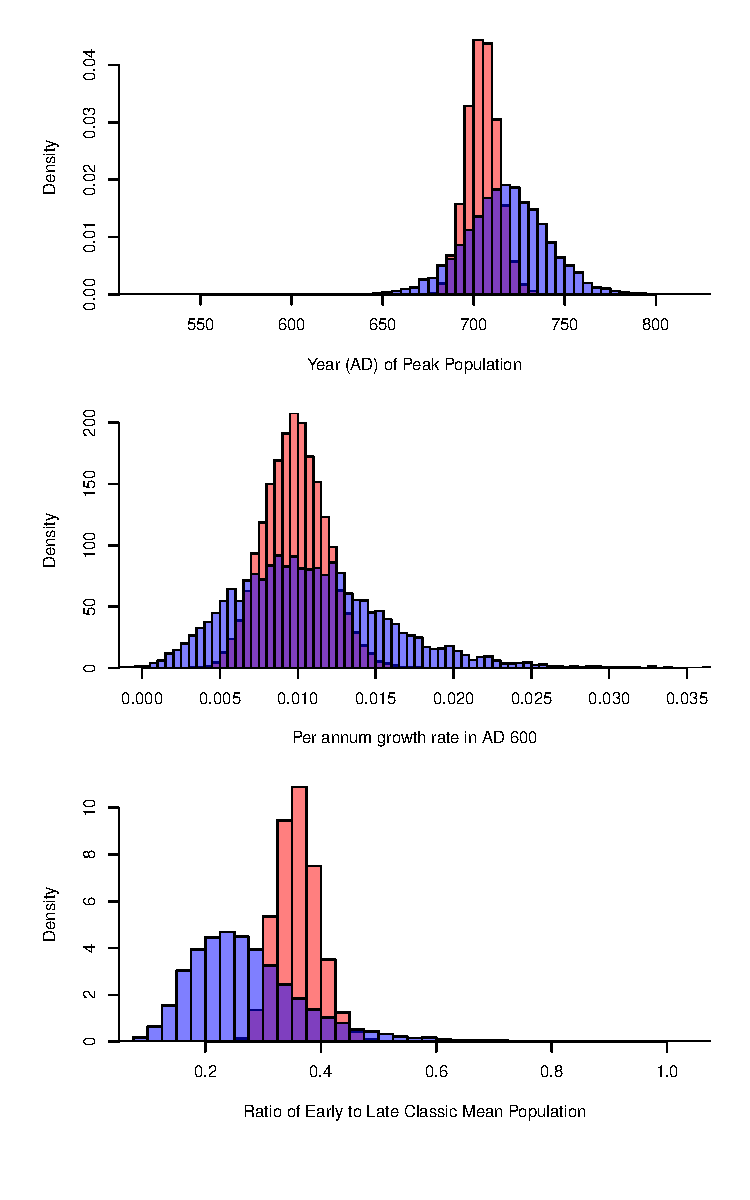
\includegraphics[height=.85\textheight]{Fig5_maya_histograms.pdf}
\end{frame}

%----------- slide --------------------------------------------------%
\begin{frame}[t]
  \frametitle{What about the bias problem?}
  Different types of data often have different bias problems
  \bigskip
  State-of-the-art improvements in reconstructing past demography demand effective fusion of different types of data
\end{frame}

%----------- slide --------------------------------------------------%
\begin{frame}
  \frametitle{Leslie Matrices}
    %\begin{block}{}
	  \begin{center}
          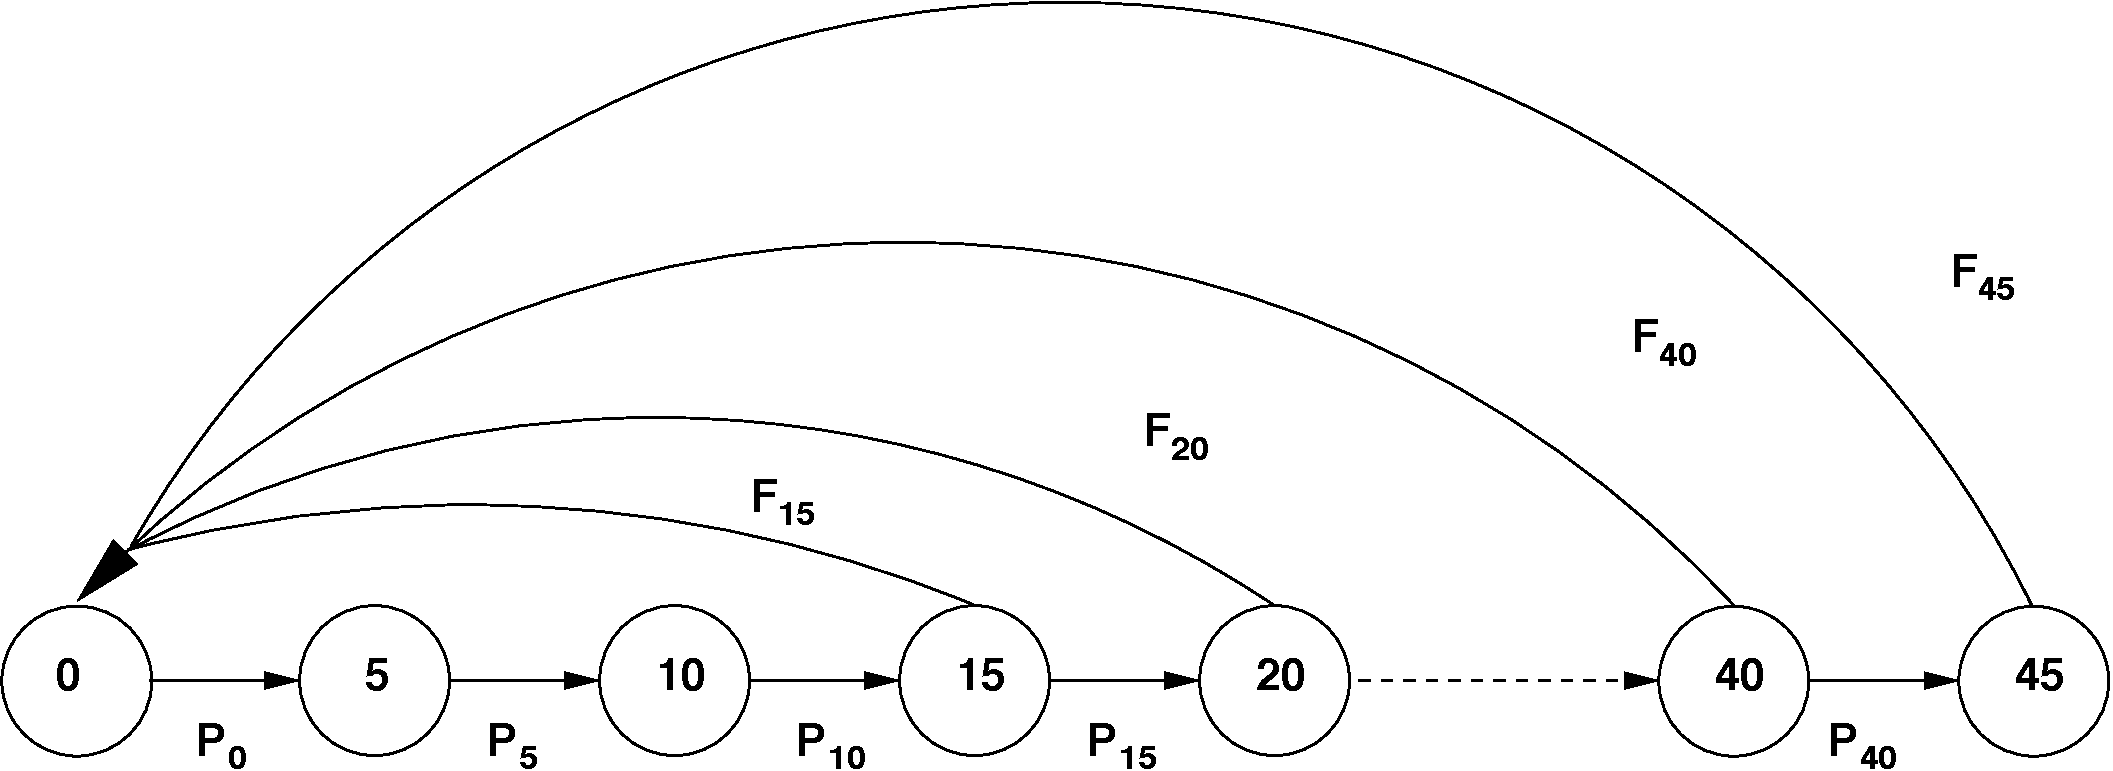
\includegraphics[width=.8\textwidth]{life-cycle.pdf}\
	  \end{center}
    %\end{block}
    \pause

    %\begin{block}{}
	  \begin{center}
	  \small
          \begin{equation*}
            \label{eq:A}
            \mathbf{A} = 
            \left( \begin{array}{cccccc}
                    F_1 & F_2 & F_3 & F_4    & \cdots  & F_{M}   \\
                    P_1 & 0   & 0   & 0      & \cdots  & 0       \\
                    0   & P_2 & 0   & 0      & \cdots  & 0       \\
                    0   & 0   & P_3 & 0      & \cdots  & 0       \\
                    0   & 0   & 0   & \ddots & \cdots  & 0       \\
                    0   & 0   & 0   & \ddots & P_{M-1} & 0
                   \end{array} \right)
          \end{equation*}
	  \end{center}
    %\end{block}

 %     $\mathbf{z}_{t+1} = \mathbf{A} \, \mathbf{z}_{t}$\\
\end{frame}

%----------- slide --------------------------------------------------%
\begin{frame}[t]
  \frametitle{Leslie Matrices}
\begin{minipage}{0\linewidth}
\begin{flushleft}                           
\begin{equation*}
      \mathbf{z}_{n+1} = \mathbf{A} \, \mathbf{z}_{n}
\end{equation*}
\pause
\begin{equation*}
	\mathbf{z}_{n} = \mathbf{A} \cdots \mathbf{A} \, \mathbf{A} \, \mathbf{z}_{0} = \mathbf{A}^t \, \mathbf{z}_{0}
\end{equation*}
\pause
\begin{equation*}
	\mathbf{z}_{n} = \mathbf{A}_n \cdots \mathbf{A}_2 \, \mathbf{A}_1 \, \mathbf{z}_{0} = {}^n_1\mathbf{Y} \, \mathbf{z}_{0}
\end{equation*}
\pause
\\
\begin{equation*}
	{}^n_1\mathbf{Y}(\greekbf{\theta}) \longrightarrow p(y,a|\greekbf{\theta})
\end{equation*}
\end{flushleft} 
\end{minipage}
\end{frame}

%----------- slide --------------------------------------------------%
\begin{frame}[t]
  \frametitle{Future Work: Radiocarbon + Age-at-Death}
    \large High growth rate implies many young people \normalsize\\
    \pause
    \bigskip
    \large Lack suitable datasets [to my knowledge]\\
    \pause
    \bigskip
    \large Need better statistical methodologies for inferring age-at-death from skeletons\\
    \pause
    \bigskip
    \large A promising PhD project, perhaps!\\
\end{frame}

\end{document}
